\documentclass[wi]{zut}

\usepackage{microtype}
\usepackage{wrapfig}

\author{Karol Działowski}
\title{Pytania na obronę pracy magisterskiej}

\makemetadata

\begin{document}

\maketitle
\tableofcontents

\section{Wstęp}

Poniższe opracowania były opracowywane indywidualnie i nie są oficjalnymi ani sprawdzonymi odpowiedziami na pytania. Na wiele pytań nie jestem pewien udzielonej odpowiedzi -- przy nich widnieje znak zapytania jak na przykładzie niżej.

W tym akapicie przedstawiony jest schemat oznaczenia pytań co do których odpowiedzi nie mam pewności. Po prawej stronie będzie wklejona ikona znaku zapytania.
\question

Podczas opracowywania pytań starałem się tłumaczyć możliwie jak najogólniej powiązane zagadnienia. W wielu przypadkach też zamieściłem odnośniki do źródeł z których korzystałem podczas tworzenia z tego dokumentu.

Zachęcam do składania poprawek poprzez stworzenie pull-requestów na repozytorium, które dostępne jest pod adresem \url{https://github.com/karlosos/ZUT_pytania_magisterskie}.

\section{Przedmioty wspólne}

\subsection{Zasady cyfryzacji sygnałów. Prawo Kotielnikowa-Shannona. Granica Nyquisa. Aliasing.}
% Aleksandr Cariow. Cyfrowe przetwarzanie sygnałów.

Pierwszy etap procesu przekształcania postaci analogowej w cryfrową to \textbf{próbkowanie}. Jest to metoda zapisu chwilowych wartości sygnału ciągłego. Największe znaczenie w procesie próbkowania ma częstotliwość pobierania próbek.

\paragraph{Twierdzenie Nyquista} definiuje minimalną częstotliwość niezbędną w celu osiągnięcia precyzyjnej reprezentacji sygnału analogowego. Rozszerzeniem tego twierdzenia jest \textbf{prawo Kotielnikowa-Shannowa}, które mówi, że w celu osiągnięcia dokładnej reprezentacji sygnału analogowego minimalna częstotliwość próbkowania powinna być co najmniej dwa razy wyższa od składowej o najwyższej częstotliwości sygnału oryginalnego. Ta minimalna częstotliwość jest często nazywana częstotliwością Nyquista lub \textbf{granicą Nyquista}.

W przypadku, gdy częstotliwość próbkowania jest mniejsza od granicy Nuqyista, to pasma częstotliwościowe nakładają się na siebie. Wywołuje to interferencję sygnału wyjściowego i efekt ten nazywany jest \textbf{aliasingiem} (utożsamianiem). Aby radzić sobie z aliasingiem możemy wykorzystać wyższą częstotliwość próbkowania lub filtr dolnoprzepustowy (antyaliasingowy)~\cite{Cariow_3}.

\begin{figure}[H]
    \centering
    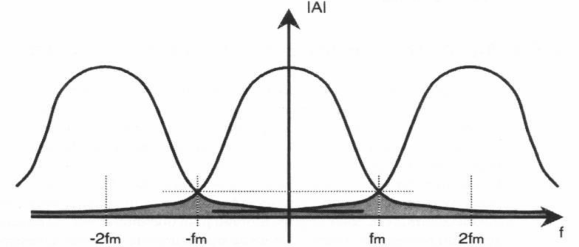
\includegraphics[width=0.7\linewidth]{images/aliasign.png}
    %\vspace{1em}
    \caption{Poszczególne pasma zachodzą na siebie i w sygnale wyjściowym wytwarzany jest aliasing.}
    \label{fig:aliasign}
    \source{Cyfrowe Przetwarzanie Sygnałów, Wykład 3 \cite{Cariow_3}}
\end{figure}


\subsection{Bezpieczny schemat podpisu cyfrowego. Modele bezpieczeństwa.}
% Tomasz Hyla. Kryptologia.

W wykładach z kryptologii brak bezpośredniej odpowiedzi na to pytanie, albo przynajmniej jej nie znalazłem. Poniższy tekst więc jest raczej wzięty na logikę i chłopski rozum niż oparty na informacjach z wykładów.

\begin{figure}[H]
    \centering
    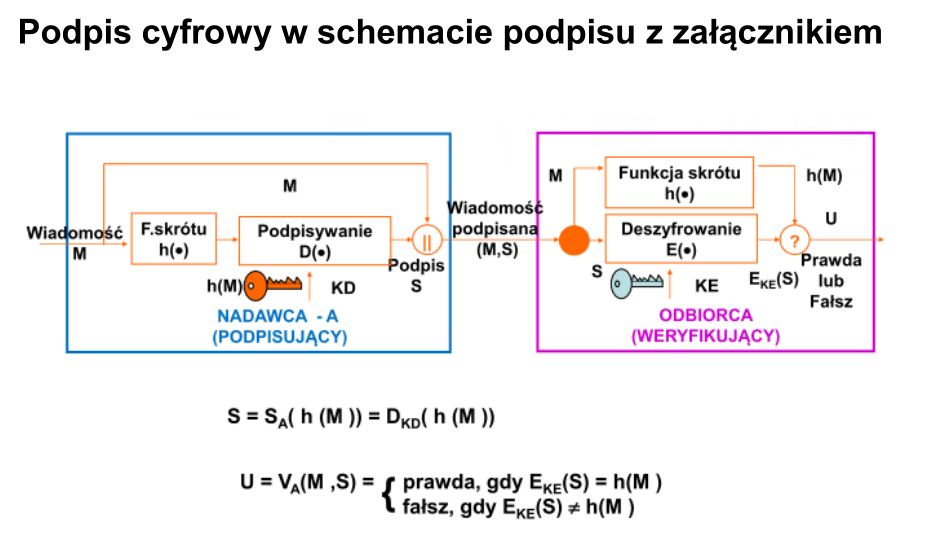
\includegraphics[width=0.7\linewidth]{images/podpis_cyfrowy.png}
    %\vspace{1em}
    \caption{Schemat podpisu cyfrowego.}
    \label{fig:digital_signature}
    \source{Kryptologia część 5 \cite{Chocian2020}}
\end{figure}

\begin{figure}[H]
    \centering
    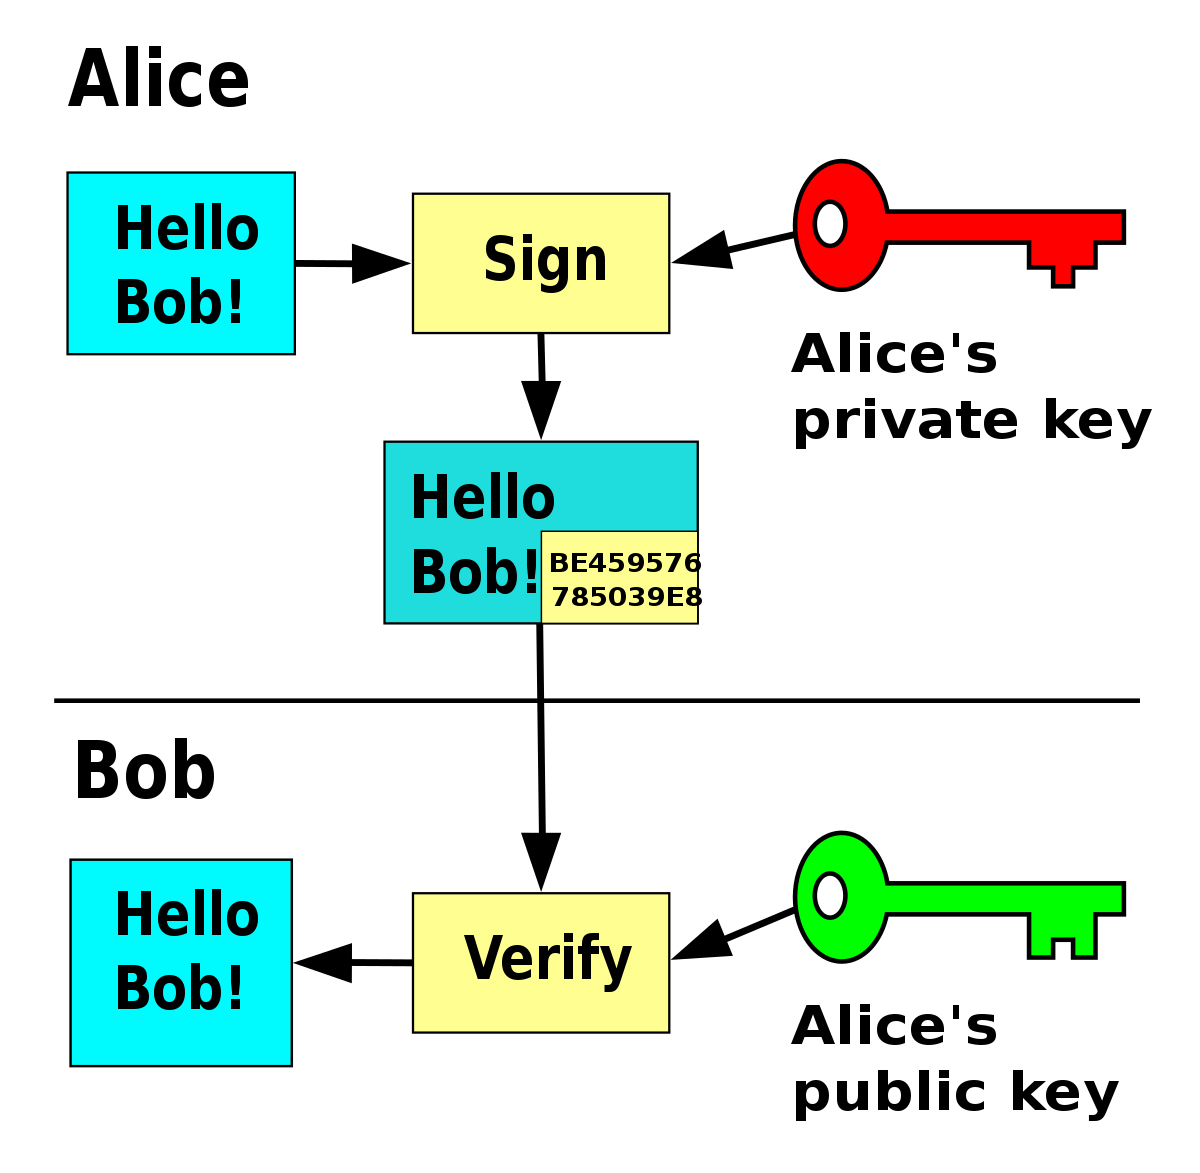
\includegraphics[width=0.5\linewidth]{images/1200px-Private_key_signing.svg.png}
    %\vspace{1em}
    \caption{Schemat podpisu cyfrowego.}
    \label{fig:digital_signature}
    \source{Wikimedia \url{https://upload.wikimedia.org/wikipedia/commons/thumb/7/78/Private_key_signing.svg/1200px-Private_key_signing.svg.png}}
\end{figure}

Podpisy cyfrowe realizowane są w oparciu o kryptografię asymetryczną. Klucz prywatny jest używany do składania podpisu, zaś klucz publiczny służy do weryfikacji. Podpis cyfrowy zapewnia autentyczność. Bezpieczeństwo podpisu zależy całkowicie od tego czy klucz prywatny jest tajny i klucz publiczny faktycznie należy do nadawcy.

% TODO: Co to znaczy ze podpis jest bezpieczny?

Właściwości bezpieczeństwa informacji (nie modele bezpieczeństwa) to poufność, integralność, osiągalność, autentyczność, rozliczalność, niezaprzeczalność (CIA - confidentiality, integrity, availability) \cite{Pejas}.

\question

\subsection{Idea interpolacji funkcji z wykorzystaniem funkcji sklejanych.}
% Piotr Piela. Matematyka obliczeniowa.

\paragraph{Funkcje sklejane} są realizacją idei gładkiej interpolacji lokalnej wielomianem niskiego stopnia z gładkim połączeniem (sklejaniem) poszczególnych wielomianów lokalnych. Mówiąc prościej jest to po prostu sklejenie kilku wielomianów w przedziałach, tak aby przybliżenie było ciągłe \cite{Piela}.

\begin{figure}[H]
    \centering
    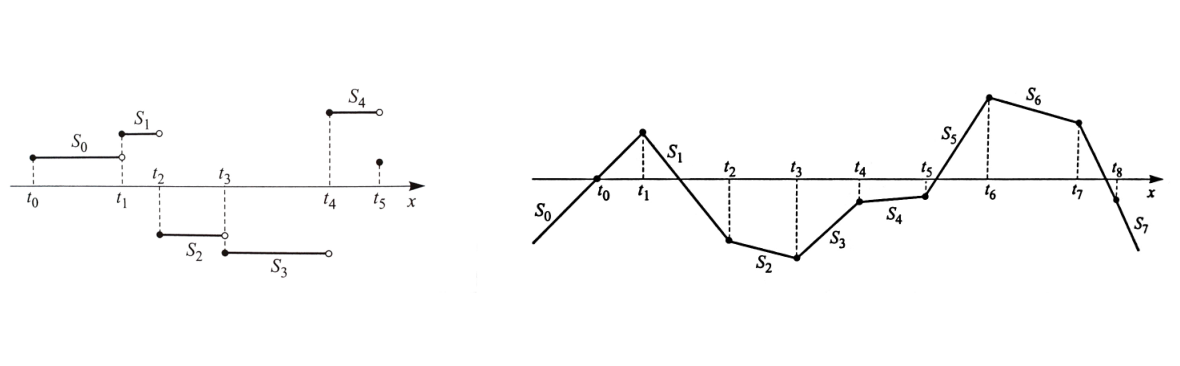
\includegraphics[width=0.8\linewidth]{images/spline.png}
    %\vspace{1em}
    \caption{Przykładu funkcji sklejanych. Funkcja sklejana stopnia 0 jest przedziałami stała, a stopnia 1 to krzywa łamana.}
    \label{fig:spline}
    \source{Matematyka obliczeniowa: W07 - Interpolacja \cite{Piela}}
\end{figure}


\begin{figure}[H]
    \centering
    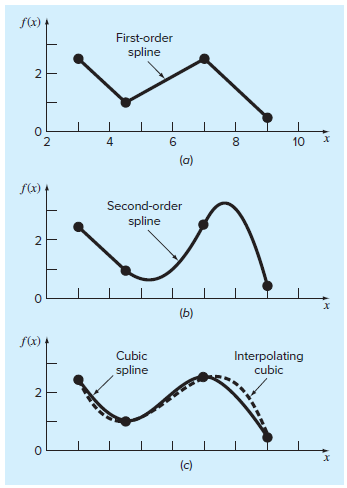
\includegraphics[width=0.4\linewidth]{images/spline2.png}
    %\vspace{1em}
    \caption{Przykłady funkcji sklejanych.}
    \label{fig:spline2}
    \source{\url{https://media.cheggcdn.com/study/d5c/d5ce9820-0f41-4ee8-8f71-39cf222db1e5/722820-18-6IP10.png}}
\end{figure}

\subsection{Styl poznawczy (kognitywny) człowieka}
% Izabela Rejer. Wprowadzenie do kognitywistyki.

Style poznawcze to trwałe różnice indywidualne w formach organizowania i \textbf{przetwarzania informacji zewnętrznych oraz doświadczenia indywidualnego}. Jest to ustabilizowany system reguł, środków psychologicznych, które człowiek świadomie lub nieświadomie stosuje w celu skutecznego równoważenia swej indywidualności z wymogami otoczenia. Reguły te odnosić się mogą do różnych aspektów regulacji psychicznej~\cite{bator1991wyznaczniki}.

Styl poznawczy to preferowany przez jednostkę sposób odbierania, przetwarzania i wykorzystywania informacji, kształtujący się w oparciu o właściwą jednostce bazę neuralną i przebieg indywidualnego doświadczenia, a przejawiający się w sytuacjach swobodnego wyboru~\cite{bator1991wyznaczniki}.

Najczęściej analizowane cechy stylów poznawczych to: refleksyjność-impulsywność, abstrakcyjność - konkretność, zależność - niezależność. Wyróżnia się strategie poznawcze takie jak:

\begin{itemize}
    \item analityczna (lokalna) i globalna,
    \item intuicyjna i racjonalna,
    \item postępowa (liberalna) i konserwatywna,
    \item słowna i obrazowa.
\end{itemize}

Podsumowując style poznawcze to opis tego, jak indywidualni ludzie postrzegają i odbierają otaczający ich świat/informacje/wiedzę. Poznanie stylów poznawczych pozwala lepiej organizować sobie warunki w których działamy i zwiększa skuteczność komunikacji pomiędzy ludźmi~\cite{perso_style}.


\subsection{Korzyści wynikające z zastosowania grafowych baz danych do przetwarzania dużych zbiorów danych o strukturach grafowych}
% Przemysław Korytkowski. Duże zbiory danych.

Sieci grafowe są wykorzystywane w zadaniach, gdzie praca na strukturach grafowych jest bardziej korzystna od tradycyjnych baz relacyjnych. Są to najczęściej problemy, które charakteryzują się dużą liczbą połączeń pomiędzy elementami (dużą liczbą relacji). Relacje te są priorytetowym elementem grafowych baz danych.

Korzyścią korzystania z takich baz jest większa wydajność dla danych o wielu asocjacjach (połączeniach, relacjach). \textbf{W bazach grafowych nie korzysta się z łączenia tabel jak w przypadku tradycyjnych baz relacyjnych.} Inną korzyścią jest łatwiejsza reprezentacja niektórych problemów za pomocą struktury grafowej.

Bazy grafowe są chętnie wykorzystywane w aplikacjach społecznościowych (modelując połączenia pomiędzy użytkownikami), w aplikacjach do rekomendacji produktów, wyznaczania ścieżek czy tras (autobusowych, lotniczych)~\cite{grafowe}. 

Zastosowania to: Sieci społecznościowe, wyznaczanie tras, usługi oparte na lokalizacji, systemy rekomendacyjne, związki chemiczne, układy biologiczne, struktury lingwistyczne i inne struktury grafowe~\cite{Jankowski2020_grafowe}.

Przykładem grafowej bazy danych jest \emph{Neo4j} z językiem zapytań \emph{Cypher}.

\subsection{Założenia i obszary zastosowania platformy Apache Spark}
% Przemysław Korytkowski. Duże zbiory danych.

Apache Spark to platforma programistyczna do obliczeń rozproszonych. Dostarcza wydajny i skalowalny silnik przetwarzania danych o dużych rozmiarach. Jest rozwinięciem idei z Hadoop MapReduce zapewniającym większą wydajność i większe możliwości analityczne~\cite{Malachowski_spark}.

Spark jest skalowalny, bo dzieli obliczenia na zadania i rozprasza je po węzłach klastra. Potrafi sam zarządzać klastrem danych. Szybka wydajność wynika z wykorzystania pamięci RAM w przeciwieństwie do bazującego na zapisach na dysku Hadoop MapReduce~\cite{Malachowski_spark}.

Spark jest napisany w języku Scala. Inne obsługiwane języki to Python i Java.

Główną ideą spark jest RDD (Resilient Distributed Dataset) - model rozproszonych danych. Metody obliczeniowe przyjmują na wejściu obiekty RDD i wynikiem ich przetwarzania jest zredukowany obiekt RDD~\cite{Malachowski_spark}.

Apache Spark wykorzystywany jest w systemach rekomendacyjnych (Spotify, Netlifx), w systemach e-commerce (Allegro), w przetwarzaniu danych strumieniowych, uczeniu maszynowym, fog computing (IoT).

\subsection{Sposoby sprawdzenia właściwości losowych danego ciągu}
% Tomasz Hyla. Kryptologia.

Testy generatorów ciągów losowych:

\begin{itemize}
    \item Test pojedynczych bitów - monobit test
    \item Test ,,pokerowy''
    \item Test ,,długich podciągów identycznych ciągów''
    \item Test ,,podciągów identycznych ciągów''
    \item Dieharder
    \item NIST Statistical Test Suite \cite{Chocian2020_2}
\end{itemize}

\paragraph{Test pojedynczych bitów - \emph{monobit test}}

Wygenerować ciąg binarny o długości 20000 bitów. \textbf{Należy określić liczbę $X$ wszystkich bitów o wartości $1$ występujących w badanym ciągu.} Wynik testu jest pomyślny gdy, $9725 < X < 10275$.

\paragraph{Test ,,pokerowy''}

Wygenerować ciąg binarny o długości 20000 bitów. \textbf{Podzielić badany ciąg na 4-bitowe paczki obejmujące 4 kolejne bity (takich paczek jest 5000)}. Zliczyć częstości $f(i)$ pojawiania się każdej z możliwych 16 sekwencji bitowych. Obliczyć wielkość $X = (16/5000) \sum{f(i)^2} - 5000$. Wynik testu jest pomyślny, gdy $2.16 < X < 46.17$.

\paragraph{Test ,,długich podciągów identycznych ciągów'' (Long runs test)}

Wygenerować ciąg binarny o długości 20000 bitów.  Jeżeli w badanym ciągu istnieje co najmniej jeden podciąg o długości $>26$ bitów zaweirający same 0 lub same 1, to wynik testu jest negatywny.

\paragraph{Test ,,podciągów identycznych ciągów'' (Runs test)}

Zliczyć wszystkie podciągi składające się tylko z bitów o wartości 0, albo tylko z bitów o wartości 1. Podzielić te podciągi na 6 grup: pierwszą - zawierającą podciągi u długości 1 bita, drugą - zawierającą podciągi o długości 2 bitów, itd.

Jeżeli liczebność którejkolwiek z sześciu grup podciągów nie mieści się w zakresie podanym w tablicy, to wynik testu jest negatywny~\cite{Chocian2020_2}.

\begin{table}[H]
\centering
\begin{tabular}{@{}rc@{}}
\toprule
Indeks paczki & Zakres    \\ \midrule
1             & 2315-2685 \\
2             & 1114-1386 \\
3             & 527-723   \\
4             & 240-384   \\
5             & 103-209   \\
6+            & 103-209   \\ \bottomrule
\end{tabular}
\end{table}

\subsection{Filtracja cyfrowa: filtry SOI i NOI}
% Aleksandr Cariow. Cyfrowe przetwarzanie sygnałów.

Wyróżniamy dwie postaci filtrów cyfrowych: (1) filtry o skończonej odpowiedzi impulsowej (SOI) (ang. finite impulse response (FIR)) i (2) filtry o nieskończonej odpowiedzi impulsowej (NOI) (ang. infinite impulse response IIR)~\cite{Cariow_7}.

Filtry SOI o skończonej odpowiedzi impulsowej to najprostszy typ filtru. Jest to splot sekwencji wejściowej ze współczynnikami filtru. Czyli jest to suma iloczynów elementów dwóch ciągów, gdzie jeden ciąg jest odwrócony~\cite{Cariow_7}.

\begin{equation}
    y_{n}=\sum_{-N}^{+N} a_{k} x_{n-k}
\end{equation}

W filtrach NOI do wyznaczenia wartości wyjściowych wykorzystuje się nie tylko dane wejściowe ale również wartości wyjściowe. Głównym założeniem i różnicą względem filtrów SOI jest to, że filtry NOI zawsze wymagają sprzężenia zwrotnego~\cite{Cariow_7}.

W odróżnieniu od filtrów SOI w filtrach tego typu każdy element sekwencji wyjściowej zależy od wartości bieżących oraz poprzednich elementów sekwencji wejściowej zarówno jak i od wartości poprzednich elementów sekwencji wyjściowej~\cite{Cariow_7}.

Jeżeli sekwencja wejściowa filtru tego typu stałaby się nagle ciągiem wartości zerowych, to sekwencja wyjściowa mogłaby (i to w pewnych warunkach już na zawsze) pozostać ciągiem elementów niezerowych~\cite{Cariow_7}.

\begin{equation}
    y_{n}=\sum_{0}^{N} a_{k} x_{n-k}+\sum_{1}^{M} b_{k} y_{n-k}
\end{equation}

Aczkolwiek pojawienie się niestabilności jest możliwe w filtrach NOI, to mają one taką zaletę, że dla takiej samej charakterystyki nachylenia wymagają mniejszej liczby odprowadzeń, niż filtry SOI~\cite{Cariow_7}.

Oznacza to, że \textbf{jeśli nasze zasoby obliczeniowe są ograniczone, możemy zastosować filtr NOI} zwracając jednak baczną uwagę na staranne zaprojektowanie jego stabilności~\cite{Cariow_7}.

Filtry NOI są powszechnie stosowane przy realizacji sprzężeń międzyukładowych dla prądu zmiennego oraz w celu wygładzania (uśredniania) przebiegów~\cite{Cariow_7}.

Najczęściej jednak wykorzystywane są łączone struktury filtrów SOI i NOI~\cite{Cariow_7}.

\subsection{Reprezentacja sygnałów za pomocą szeregów funkcyjnych. Dyskretne transformacje ortogonalne oraz szybkie algorytmy ich wyznaczania.}
% Aleksandr Cariow. Cyfrowe przetwarzanie sygnałów.

Sygnały $x(n)$ o złożonym kształcie reprezentuje się jako liniowe kombinacje prostszych przebiegów. Wykonuje się to za pomocą doboru zestawu z góry określonych funkcji $b_0(n), b_1(n), \ldots, b_k(n)$ oraz pewnych współczynników liczbowych $c_0, c_1, \ldots, c_k$. Wtedy sygnał $x(n)$ zdefiniowany za pomocą $N$ próbek z numerami $0, 1, \ldots, N-1$ można przedstawić w postaci:

\begin{equation}
    x(n)=\sum_{k=0}^{\infty} c_{k} b_{k}(n)
\end{equation}

\begin{equation}
    c_{k}=\mathrm{E}_{k}^{-1} \sum_{n=0}^{N-1} x(n) b_{k}(n)
\end{equation}

Możliwe jest przechodzenie pomiędzy dziedziną czasową a widmem za pomocą dyskretnych transformacji w odpowiedniej bazie. Czyli sygnał cyfrowy można zdefiniować za pomocą jego próbek w dyskretnych chwilach czasu lub za pomocą zbioru współczynników widmowych~\cite{Cariow_6}.

Ważne jest aby zbiór funkcji bazowych spełniał następujące warunki:

\begin{enumerate}
    \item Funkcje bazowe powinny być liniowo niezależne
    $$a_{0} b_{0}(n)+a_{1} b_{1}(n)+\ldots+a_{N-1} b_{N-1}(n) \neq 0$$
    \item System musi być uporządkowany. To oznacza że w zbiorze indeksów ma miejsce relacja porządku określająca jaka z funkcji jest poprzedzająca i jaka jest następna.
    \item Funkcje bazowe na przedziale ortogonalności powinny posiadać skończoną energię.
    \item System funkcji powinien tworzyć rodzinę zupełną - to znaczy, że niemożliwe jest dodanie ani jednej funkcji, która byłaby ortogonalna względem reszty wszystkich funkcji systemu.
\end{enumerate}

Najczęściej jako bazę wybiera się zbiór liniowo niezależnych funkcji ortogonalnych, dla których spełniony jest warunek:

\begin{equation}
    \sum_{n=0}^{N-1} b_{k}(n) \cdot b_{l}^{*}(n)=0, \quad k \neq l
\end{equation}

Wyróżnione transformacje ortogonalne:

\begin{enumerate}
    \item Baza funkcji Walsha - funkcje schodkowe
    \item Szybkie transformaty w Bazie funkcji Vilenkina:
    \begin{enumerate}
        \item Vilenkina-Pontryagina (VPF)
        \item Vilenkina-Kroneckera (VKF)
        \item Vilenkina-Walsha
    \end{enumerate}
    \item Baza funkcji Haara
    \item Baza funkcji piłopodobnych (Slant function)
    \item Dyskretne Przekształcenie Kosinusowe (DCT) - algorytm Arai, Agui i Nakajama
    \item Baza funkcji Hartley'a~\cite{Cariow_6}.
\end{enumerate}

\subsection{Atak na podpis cyfrowy wykorzystujący paradoks dnia urodzin}
% Tomasz Hyla. Kryptologia.

Paradoks dnia urodzin odnosi się do prawdopodobieństwa tego, że w zbiorze $n$ losowo wybranych ludzi będzie para, która ma urodziny tego samego dnia. W grupie liczącej 23 osoby to prawdopodobieństwo wynosi 50\%, a grupa 70 osób ma 99.9\% prawdopodobieństwa występowania takiej pary \cite{wiki:Birthday_problem}.


\begin{figure}[H]
    \centering
    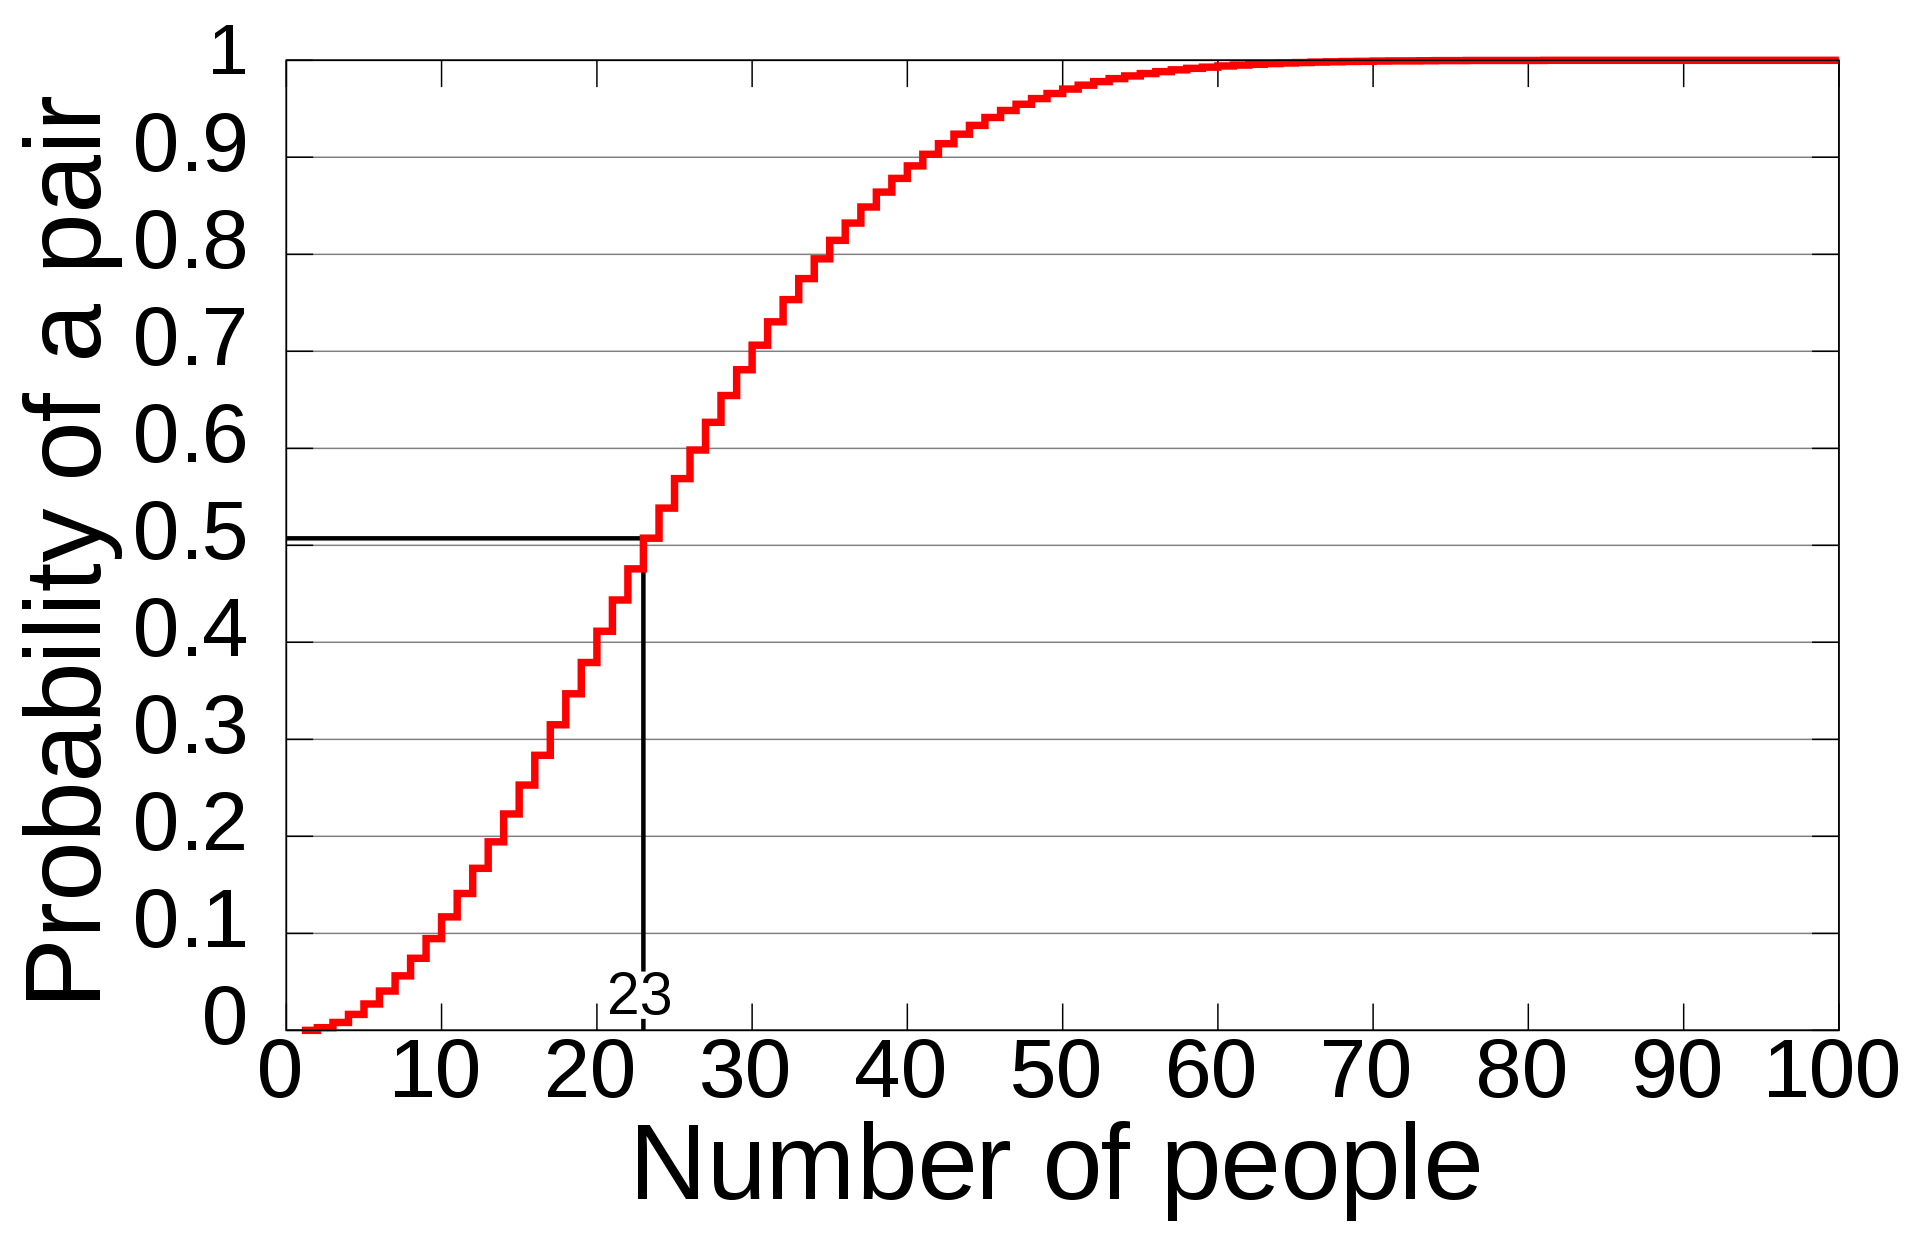
\includegraphics[width=0.5\linewidth]{images/Birthday_Paradox.svg.png}
    %\vspace{1em}
    \caption{Obliczone prawdopodobieństwo, ze co najmniej dwie osoby mają wspólną datę urodzenia.}
    \label{fig:birthdaj}
    \source{\url{https://www.wikiwand.com/en/Birthday_problem} \cite{wiki:Birthday_problem}}
\end{figure}

Podpisy cyfrowe mogą być podatne na atak wykorzystujący paradoks dnia urodzin (ang. birthday attack). Zazwyczaj podpisywanie wiadomości $m$ zaczyna się od obliczenia $f(m)$, gdzie $f$ to kryptograficzna funkcja skrótu a następnie używa się tajnego klucza do podpisu $f(m)$ (wartości skrótu z wiadomości). Załóżmy że adwersarz, chce wrobić Boba w podpis nieuczciwego dokumentu. Adwersarz przygotowuje uczciwy dokument $m$ i nieuczciwy $m'$. Uczciwy dokument $m$ jest tak modyfikowany (np. dodawane białe znaki) aby jego skrót był równy skrótowy z dokumentu $m'$, czyli $f(m) = f(m')$~\cite{wiki:Birthday_problem}.

W takiej sytuacji, gdy Bob podpisze dokument $m$ będzie to równoważne z podpisaniem $m'$.

Aby obronić się przed tym atakiem, długość skrótu powinna być stosunkowo duża, aby znalezienie kolizji było wystarczająco trudne. Innym sposobem na przeciwdziałanie temu atakowi, jest mała zmiana dokumentu przez Boba przed podpisaniem (ale wtedy adwersarz może tak samo szukać kolizji zmieniając fałszywy dokument)~\cite{wiki:Birthday_problem}.

Na wykładach atak ten był przedstawiony w trochę inny sposób. Podpis cyfrowy dla wiadomości $m$ to $s = D_d(h(m))$, gdzie $D_d$ to klucz prywatny Boba, $h$ to funkcja skrótu. Mając skrót o długości $n$ bitów należy:

\begin{itemize}
    \item wygenerować $2^{n/2}$ fałszywych wiadomości $m_i$
    \item wygenerować $2^{n/2}$ fałszywych podpisów $s_i$
    \item znaleźć taką parę, że $E_e(s_j) = h(m_k)$, gdzie $E$ to klucz publiczny Boba \cite{Chocian2020}.
\end{itemize}

\subsection{Podział metod rozwiązywania równań liniowych metodami numerycznymi}
% Piotr Piela. Matematyka obliczeniowa.

Układem równań liniowych nazywamy układ:
$$
\left\{\begin{array}{l}
a_{11} x_{1}+a_{12} x_{2}+\ldots+a_{1 n} x_{n}=b_{1} \\
a_{21} x_{1}+a_{22} x_{2}+\ldots+a_{2 n} x_{n}=b_{2} \\
\cdots \\
a_{m 1} x_{1}+a_{m 2} x_{2}+\ldots+a_{m n} x_{n}=b_{m}
\end{array}\right.
$$
Ten sam układ zapisany w postaci macierzowej:
$$
\left(\begin{array}{cccc}
a_{11} & a_{12} & \ldots & a_{1 n} \\
a_{21} & a_{22} & \ldots & a_{2 n} \\
\vdots & \vdots & \vdots & \vdots \\
a_{m 1} & a_{m 2} & \ldots & a_{m n}
\end{array}\right) \cdot\left(\begin{array}{c}
x_{1} \\
x_{2} \\
\vdots \\
x_{n}
\end{array}\right)=\left(\begin{array}{c}
b_{1} \\
b_{2} \\
\vdots \\
b_{m}
\end{array}\right)
$$

\textbf{Metody rozwiązywania} układów równań liniowych~\cite{Piela_URL}:

\begin{itemize}
    \item Wzory Cramera
    \item Odwracane Macierzy
    \item Metody eliminacji
    \begin{itemize}
        \item Metoda eliminacji Gaussa
        \item Metoda eliminacji Gaussa-Crouta
        \item Metoda eliminacji Jordana
    \end{itemize}
    \item Metody wykorzystujące rozkłady macierzy
    \begin{itemize}
        \item Rozkład LU
        \item Rozkład QR
        \item Rozkład SvD
    \end{itemize}
    \item Metody iteracyjne
    \begin{itemize}
        \item Metoda Richardsona
        \item Metoda Jacobiego
        \item Metoda Gaussa-Seidela
        \item Metoda nadrelaksacji (SOR)
    \end{itemize}
\end{itemize}

\subsection{Algorytm numeryczny niestabilny a algorytm źle uwarunkowany}
% Piotr Piela. Matematyka obliczeniowa.

Algorytm numeryczny nazywamy \textbf{niestabilnym} jeśli małe błędy popełnione na jakimś etapie obliczeń rosną w następnych etapach i poważnie zniekształcają ostateczne wyniki. Przy badaniu stabilności wykorzystuje się błędy względne~\cite{Piela_Wstep}.

Algorytm numeryczny jest \textbf{źle uwarunkowany} jeśli małe zmiany danych początkowych wywołują duże zmiany wyników. Dla pewnych typów zadań można określić wskaźnik uwarunkowania, który charakteryzuje wpływ zaburzeń danych na otrzymane wyniki. Jeśli jest on duży to zadanie jest źle uwarunkowane. Uwarunkowanie jest cechą samego zadania i nie jest związane z metodą jego rozwiązania~\cite{Piela_Wstep}.

\subsection{Programowanie kodu wielowątkowego wraz z wzajemnym wykluczaniem w C++ 11 Threads}
% Marek Pałkowski. Obliczenia dużej mocy.

Wraz z standardem C++11 wprowadzono do biblioteki standardowej moduł do zarządzania wątkami, instrukcjami warunkowymi czy mutexami (mutexy służą do zapewnienia ochrony przed jednoczesnym dostępem do danych, jest to mechanizm wzjamnego wykluczania). Dokumentacja dostępna jest pod adresem \url{https://en.cppreference.com/w/cpp/thread}.

Dzięki temu nie trzeba korzystać z wątków z biblioteki \lstinline{pthreads}, która była przeznaczona do języka C.

\code{Przykład tworzenia wątków z wykorzystaniem C++11 threads.}
{\url{https://www.bogotobogo.com/cplusplus/C11/1_C11_creating_thread.php}}{\label{kod:przyklad}}
\begin{lstlisting}[language=C++]
#include <iostream>
#include <thread>

void thread_function()
{
    std::cout << "thread function\n";
}

int main()
{
    std::thread t(&thread_function);   // t starts running
    std::cout << "main thread\n";
    t.join();   // main thread waits for the thread t to finish
    return 0;
}
\end{lstlisting}

Inną możliwością jest tworzenie wątków przy wykorzystaniu wyrażenia lambda.

\code{Przykład tworzenia wątków z wykorzystaniem mutexów.}
{\url{https://en.cppreference.com/w/cpp/thread/mutex}}{\label{kod:przyklad}}
\begin{lstlisting}[language=C++]
#include <iostream>
#include <map>
#include <string>
#include <chrono>
#include <thread>
#include <mutex>
 
std::map<std::string, std::string> g_pages;
std::mutex g_pages_mutex;
 
void save_page(const std::string &url)
{
    // simulate a long page fetch
    std::this_thread::sleep_for(std::chrono::seconds(2));
    std::string result = "fake content";
 
    std::lock_guard<std::mutex> guard(g_pages_mutex);
    g_pages[url] = result;
}
 
int main() 
{
    std::thread t1(save_page, "http://foo");
    std::thread t2(save_page, "http://bar");
    t1.join();
    t2.join();
 
    // safe to access g_pages without lock now, as the threads are joined
    for (const auto &pair : g_pages) {
        std::cout << pair.first << " => " << pair.second << '\n';
    }
}
\end{lstlisting}

\subsection{Cechy środowiska Hadoop}
% Przemysław Korytkowski. Duże zbiory danych.

Apache Hadoop to otwarta platforma programistyczna napisana w języku Java przeznaczona do \textbf{rozproszonego składowania i przetwarzania wielkich zbiorów danych przy pomocy klastrów komputerowych}. Wszystkie moduły Hadoop zostały zaprojektowane z założeniem, że awarie sprzętowe są rzeczą naturalną i powinny być automatycznie obsługiwane~\cite{Korytkowski_hadoop}.

Cechy szczególne środowiska Hadoop:

\begin{itemize}
    \item Możliwość przechowywania i szybkiego \textbf{przetwarzania ogromnej ilości danych} różnego typu
    \item \textbf{Moc obliczeniowa} - dzięki rozproszonemu modelowi obliczeniowemu przetwarzanie big data jest szybkie. Im więcej węzłów jest używanych, tym większa moc przetwarzania.
    \item \textbf{Tolerancja na błędy} - odporne na awarię sprzętu, automatyczne przekierowanie do innych węzłów, tworzenie wielu kopii danych automatycznie.
    \item \textbf{Elastyczność} - nie trzeba wstępnie przetwarzać danych przed zapisem. Można przechowywać dane nieustrukturyzowane i później zdecydować jak je wykorzystać.
    \item \textbf{Niski koszt} - jest bezpłatne, bo open source
    \item \textbf{Skalowalność} - łatwe rozbudowywanie systemu poprzez dodawanie węzłów
\end{itemize}

W porównaniu do relacyjnych baz danych w hadoopie dane nie muszą być ustrukturyzowane. Przechowywane są duże rozmiary danych. Jęzkiem zamiast SQL jest HQL. Wykorzystywany jest to przetwarzania dużej liczby danych (audio, video, logi). Charakteryzuje się wysoką wydajnością, niską integralnością (brak ACID)~\cite{Korytkowski_hadoop}.

W ekosystemie wykorzystywany jest rozproszony system plików \textbf{HDFS}. Do przetwarzania dużych ilości danych wykorzystywany jest paradygmat \textbf{MapReduce}. Za zarządzanie zasobami klastra odpowiada \textbf{YARN}~\cite{Korytkowski_hadoop}.

Nacisk na szybki zapis i elastyczność (schema-on-read)~\cite{Korytkowski_hadoop}.

\subsection{Rodzaje błędów składające się na całkowity błąd obliczeń numerycznych}
% Piotr Piela. Matematyka obliczeniowa.
Na błąd całkowity obliczeń numerycznych składają się następujące rodzaje błędów:
\begin{itemize}
    \item błąd wejścia,
    \begin{itemize}
        \item błąd wejścia dla podstawowych działań arytmetycznych, 
    \end{itemize}
    \item błąd metody,
    \begin{itemize}
        \item błąd urwania procedury iteracyjnej
        \item błąd dyskretyzacji
    \end{itemize}
    \item błąd zaokrąglenia.
\end{itemize}

\textbf{Błąd wejścia zależy od niedokładności pomiarów}, przeoczeń, błędnych odczytów, brakiem możliwości zapisu dowolnej liczby rzeczywistej w postaci liczby maszynowej~\cite{Piela_Wstep}.

\textbf{Błąd metody zależy od konieczności przybliżania wartości ciągłych}, nie zależy od błędów wejścia i zaokrąglenia, zależy od konieczności reprezentowania procesów nieskończonych~\cite{Piela_Wstep}.

Błąd dyskretyzacji powstaje w wyniku aproksymacji struktur ciągłych za pomocą układów dyskretnych (np. całkowanie numeryczne)~\cite{Piela_Wstep}.

\textbf{Błąd zaokrąglenia wynika z potrzeby reprezentowania liczb w postaci maszynowej} (na skończonej liczbie bitów). Z tego powodu powstaje zjawisko obcięcia lub zaokrąglenia.

\subsection{Standard C++ 17 Parallel}
% Marek Palkowski. Obliczenia dużej mocy.
% https://en.cppreference.com/w/cpp/17

Wraz z standardem C++17 w ramach języka został zdefiniowany standard Parallel. Polegało to na dodaniu do modułu \lstinline{algorithms} metod działających współbieżnie oraz innych funkcjonalności współbieżności (\lstinline{execution policies})~\cite{C++17}.

Przykładowe algorytmy to:

\begin{itemize}
    \item sort
    \item reduce
    \item \textbf{for\_each}
    \item count
    \item find
    \item transform\_reduce~\cite{MicrosoftCPP17}
\end{itemize}


\code{Uruchomienie algorytmu \lstinline{find} w trybie sekwencyjnym i równoległym.}
{\url{https://dev.to/fenbf/examples-of-parallel-algorithms-from-c17-3jej}}{\label{kod:przyklad}}
\begin{lstlisting}[language=C++]
auto res = std::find(std::execution::seq, std::begin(v), std::end(v), 0.6);
return res == std::end(v) ? 0.0 : 1.0;

auto res = std::find(std::execution::par, std::begin(v), std::end(v), 0.6);
return res == std::end(v) ? 0.0 : 1.0;
\end{lstlisting}


\subsection{Dokładność rozwiązywania równań różniczkowych metodami numerycznymi}
% Piotr Piela. Matematyka obliczeniowa.

Dokładność rozwiązywania równań różniczkowych zależy od:

\begin{itemize}
    \item wybranej metody (ode45, ode1, ode4, fixed step, variable step)
    \item dobranego kroku metody
\end{itemize}
\question

Wśród metod rozwiązywania RR wyróżniamy:
\begin{itemize}
    \item metode Eulera
    \item zmodyfikowaną metodę Eulera
    \item udoskonaloną metodę Eulera
    \item rodzinę metod Rungego-Kutty
    \item metodę Adams'a-Bashfort'a
\end{itemize}

Wyróżniamy metody jednokrokowe i wielokrokowe oraz ze stałym krokiem i ze zmiennym krokiem, oraz różnych rzędów~\cite{Piela_RR}.

\subsection{Wpływ zachowań z obszaru kognitywistyki relacji społecznych na rozwój mediów społecznościowych}
% Izabela Rejer. Wprowadzenie do kognitywistyki.

Brak informacji na ten temat. Można powiedzieć jaki wpływ media społecznościowe mają na rozwój kognitywistyki (bo dostarczają platformy do wielu badań). Nie wiem jaki ,,zachowania z obszaru kognitywistyki relacji spiłecznych'' miały wpływ na social-media. Nie wiem nawet co to znaczy.
\question

\subsection{Programowanie przenośnego kodu wielowątkowego na przykładzie PosixThreads}
% Marek Pałkowski. Obliczenia dużej mocy.

Posix Threads to biblioteka dedykowana do pisania aplikacji wielowątkowych zgodna z językiem C/C++. Jest przenośna, bo działa pod systemami Windows i Linux. Pozwala na tworzenie i kończenie wątków, sychronizacje, blokady, semafory i zmienne warunkowe~\cite{Palkowski_POSIX}.

Do uruchomienia nowego wątku służy funkcja \lstinline{pthread_create} do której przekazujemy wskaźnik na funkcję którą chcemy wykonać oraz parametry wywołania tej funkcji. Możemy oczekiwać na zakączenie wątku przy użyciu \lstinline{pthread_join}, gdzie podajemy identyfikator wątku~\cite{Palkowski_POSIX}.

\code{Przykład tworzenia i kończenia wątków}
{Wykład Posix Threads \cite{Palkowski_POSIX}}{\label{kod:przyklad}}
\begin{lstlisting}[language=C++]
#include <pthread.h>
#include <stdio.h>
#define NUM_THREADS     5

void *PrintHello(void *threadid)
{
   long tid;
   tid = (long)threadid;
   printf("Hello World! It's me, thread #%ld!\n", tid);
   pthread_exit(NULL);
}

int main (int argc, char *argv[])
{
   pthread_t threads[NUM_THREADS];
   int rc;
   long t;
   for(t=0; t<NUM_THREADS; t++){
      printf("In main: creating thread %ld\n", t);
      rc = pthread_create(&threads[t], NULL, PrintHello, (void *)t);
      if (rc){
         printf("ERROR; return code from pthread_create() is %d\n", rc);
         exit(-1);
      }
   }

   /* Last thing that main() should do */
   pthread_exit(NULL);
}
\end{lstlisting}

W bibliotece Posix Threads mamy też do dyspozycji obiekty mutex. Jest to mechanizm wzajemnego wykluczania służący do ochrony danych współdzielonych przed jednoczesnymi modyfikacjami. Mechanizm służy do implementacji sekcji krytycznych, semaforów i monitorów. Mutex ma dwa stany: otwarty i zamknięty~\cite{Palkowski_POSIX}.

Zmienne warunkowe są mechanizmem umożliwiającym zawieszanie i zwolnienie czasu procesora (wątku) do momentu, w którym zostanie spełniony określony warunek. Zmienna warunkowa musi być zawsze otoczona obiektem mutex, aby uniknąć jednoczesnej próby oczekiwania i sygnalizowania na zmiennej warunkowej~\cite{Palkowski_POSIX}.

\code{Przykład wykorzystania zmiennych warunkowych i mutexów}
{Wykład Posix Threads \cite{Palkowski_POSIX}}{\label{kod:przyklad}}
\begin{lstlisting}[language=C++]
int  number;
pthread_mutex_t  mutex  =  PTHREAD_MUTEX_INITIALIZER;
pthread_cond_t  cond  =  PTHREAD_COND_INITIALIZER;
void*  RandomThread(void*  arg)
{
	srandom(1);
	for  (int  i=0;  i<20;  i++)
	{
		pthread_mutex_lock(&mutex);
		number  =  static_cast<double>(rand())/RAND_MAX*10;
		if  (number  <  5)
		{
			std::cout  <<  "mniejsza";
			pthread_cond_broadcast(&cond);
		}
		pthread_mutex_unlock(&mutex);
		sleep(1);
	}
}

void*  OutputThread(void*  arg)
{
	while  (true)
	{	
		pthread_mutex_lock(&mutex);
		pthread_cond_wait(&cond,  &mutex);
		std::cout  <<  "Wygenerowana  liczba  -  "  <<  number
		<<  "  jest  mniejsza  od  5"  <<  std::endl;
		pthread_mutex_unlock(&mutex);
	}
}

int  main()
{
	pthread_t  thread1;
	if  (pthread_create(&thread1,  NULL,  RandomThread,  NULL))
	{
		std::cerr  <<  "bład  podczas  tworzenia  watku"  <<  std::endl;
		exit(1);
	}
	pthread_t  thread2;
	if  (pthread_create(&thread2,  NULL,  OutputThread,  NULL))
	{
		std::cerr  <<  "bład  podczas  tworzenia  watku"  <<  std::endl;
		exit(1);
	}
	void*  result;
	pthread_join(thread1,  &result);
	pthread_cancel(thread2);
	pthread_exit(NULL);
}
\end{lstlisting}

\subsection{Zastosowanie okulografii w pięciu wybranych dziedzinach życia}
% Izabela Rejer. Wprowadzenie do kognitywistyki.

Okulografia (ang. eye-tracking) technika śledzenia punktu skupienia wzroku, ruchów gałki ocznej oraz rozmiaru źrenicy osoby badanej \cite{wiki:Okulografia}.

Okulografia wykorzystywana jest w:

\begin{enumerate}
    \item Marketingu - w ramach badań nad tym co przykuwa uwagę konsumentów, przy projektowaniu reklam, opakowań
    \item Rozrywce (gry wideo) - wykorzystanie eye-trackingu w celach rozrywkowych, np. w grach komputerowych. Przykładem eye-trackera do zastosowań gamingowych jest \textit{Tobii Eye Tracker 5}.
    \item Badaniach nad doświadczeniem użytkownika (UX) - przy projektowaniu i testowaniu różnego rodzaju interfejsów graficznych i systemów komputerowych (przykładowo testowanie stron internetowych budując mapy ciepła, ścieżki fiksacji, itd.)
    \item Motoryzacji - wykrywanie zmęczenia, przy projektowaniu desek rozdzielczych
    \item Interfejsach człowiek komputer - w komunikacji z komputerem 
    \item Medycynie - w diagnostyce (schizofrenia, alzheimer, autyzm, ADHD, parkinson), w leczeniu
\end{enumerate}

\section{Inteligencja obliczeniowa}

\subsection{Charakterystyka języków programowania wykorzystywanych w analizie danych}
% Marcin Pluciński. Języki analizy danych.

Najczęściej wykorzystywane języki programowania wykorzystywane w analizie danych to:

\begin{itemize}
    \item Python
    \item Matlab
    \item R
\end{itemize}

Wszystkie te języki są wysokopoziomowe, dynamiczne, interpretowalne. Mają rozbudowaną bazę bibliotek ułatwiających analizę danych. Charakteryzują się szybkością prototypownia, ale niekoniecznie wydajnością.

Ostatnio dużą popularność zyskuje język Julia. Jest to język ogólnego przeznaczenia. Zbudowany specjalnie na potrzeby data science i uczenia maszynowego. Jest to język wysokiego poziomu, dynamiczne, darmowy i open-source. Składnia jest łatwa do zrozumienia. 

Zaletą Julii jest szybkość działania (lepsza od Pythona). Uzyskano to przez wykorzystanie kompilacji JIT (jist in time)\footnote{Więcej o języku Julia możesz poczytać na \url{https://julialang.org/}}. 

Za kilka lat na uczelnii studencii będą chcieli odchdodzić od Pythona na rzecz Julii, tak jak my chcieliśmy Pythona zamiast Matlaba.


\subsection{Porównanie dwóch dowolnych algorytmów wykrywania obiektów}
% Paweł Forczmański. Widzenie komputerowe.

Do problemu detekcji można wykorzystać deskryptor \textbf{HoGa (Histogram of Oriented Gradients)}. Dzielimy obraz na siatkę lokalnych gradientów dla wybranych kierunków (najczęściej 8 kierunków). Jako klasyfikator wykorzystuje się liniowy SVM~\cite{ForczmanskiCV}. Każdy piksel głosuje w ramach swojej komórki na pewien kierunek gradientu z siłą proporcjonalną do długości gradientu zaczepionego w tym pikselu.

Uśredniony deskryptor HoGa toleruje zmiany pozy, ubrania, oświetlenia i tła w przypadku detekcji sylwetek ludzkich~\cite{ForczmanskiCV}.

\begin{figure}[H]
    \centering
    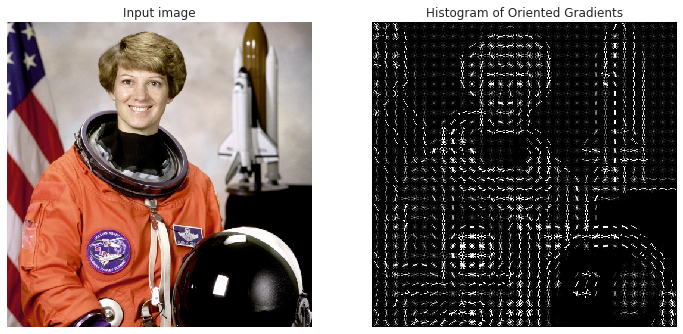
\includegraphics[width=0.7\linewidth]{images/hog-vis.png}
    %\vspace{1em}
    \caption{Deskryptor HoGa}
    \label{fig:pdgd}
    \source{\url{https://iq.opengenus.org/object-detection-with-histogram-of-oriented-gradients-hog/}}
\end{figure}

Innym algorytmem jest \textbf{AdaBoost Cascade Detector}. Jest to efektywnie obliczeniowo algorytm, który wcześnie odrzuca błędnych kandydatów. Jest to zrealizowane za pomocą łańcucha klasyfikatorów, które odrzucają pewną część przykładów, pozostawiając prawie wszystkie pozytywne~\cite{ForczmanskiCV}.

Każdy klasyfikator AdaBoost to zespół klasyfikatorów, które wykorzystują proste cechy Haara. Cecha Haara to różnica średniej jasności pomiędzy dwoma obszarami~\cite{ForczmanskiCV}.

W celu przyspieszenia obliczeń cech Haara wykorzystuje się obrazy całkowe~\cite{ForczmanskiCV}. 

Jest to najszybszy z detektorów dla obrazów w skali szarości (nie licząc nowoczesnych podejść głębokiego uczenia)~\cite{ForczmanskiCV}.

\begin{figure}[H]
    \centering
    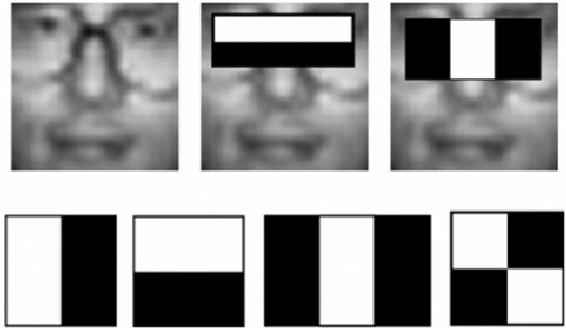
\includegraphics[width=0.5\linewidth]{images/Haar-features-used-for-Viola-Jones-face-detection-method.png}
    %\vspace{1em}
    \caption{Cechy Haara wykorzystywane w detektorze Viola-Jones (AdaBoost)}
    \label{fig:pdgd}
    \source{\url{https://www.researchgate.net/figure/Haar-features-used-for-Viola-Jones-face-detection-method_fig1_268348020}}
\end{figure}

\subsection{Charakterystyka wybranych metod śledzenia obiektów}
% Paweł Forczmański. Widzenie komputerowe.

Przykładowe trackery dostępne w \textit{OpenCV}:

\begin{itemize}
    \item CSRT
    \item KCF
    \item Boosting
    \item MedianFlow
\end{itemize}

Inne popularne trackery:

\begin{itemize}
    \item MeanShift
    \item CamShift
    \item Particle Filter
\end{itemize}

Algorytm mean-shift może być wykorzystywany do śledzenia obiektów w sekwencjach wideo. Wymaga określenia cech obrazu na której będzie operować, np. kolor, krawędzie, wynik filtra cząsteczkowego czy inne cechy. Główną zaletą Mean-shift jest jego prostota.

Największą wadą tej metody jest bazowania na wyglądzie śledzonego obiektu. Tworzy to problemy w przypadku okluzji, zmiany wyglądu poprzez rotację, zmianę skali itd.

Mean-shift polega na wyznaczeniu lokalnych ekstremów rozkładów gęstości analizowanej cechy. Procedura ma charakter iteracyjny a sam proces rozpoczyna się od wskazania śledzonego obiektu (w sposób manualny lub automatyczny). Algorytmy z rodziny mean-shift operują na rozkładzie prawdopodobieństwa, np. gdy wybraną cechą jest barwa, to zadanie jest realizowane w oparciu o histogram. Okno poszukiwań przemieszcza się wraz z rosnącym gradientem aż do momentu zbieżności.

Rozwiązaniem problemu skalowanie jest metoda CAMSHIFT, która adaptuje się do rozmiaru okna opisującego śledzony obiekt. Podstawowa różnica polega na dynamicznej adaptacji okna. 

\subsection{Trzy pytania, na które odpowiadają Ukryte Modele Markowa oraz używane do tego celu algorytmy}
% Marcin Pietrzykowski. Eksploracja danych.

Na początku warto przypomnieć co to Ukryte Modele Markowa. Model Markowa składa się z $N$ stanów $S$, które są ukryte oraz $M$ obserwacji $V$. Podobnie jak w łańcuchu Markowa w każdym momencie czasowym model może być w jednym stanie. Prawdopodobieństwa przejścia pomiędzy stanami zależą tylko od stanu poprzedniego. Dla każdego stanu system generuje obserwacje z danym prawdopodobieństwem \cite{Pietrzykowski2020}. 

Modele Markowa są dobre do rozpoznawania zmiennych wzorców, np. mowa, pismo odręczne, gesty, predykcja genów itd.\cite{Pietrzykowski2020}

\begin{figure}[H]
    \centering
    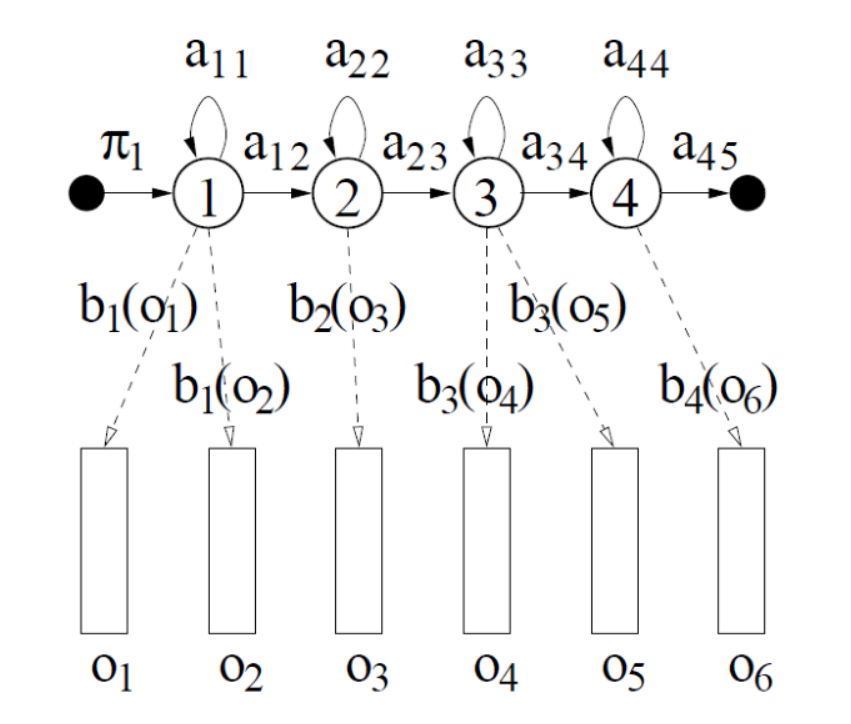
\includegraphics[width=0.5\linewidth]{images/hidden_markov.png}
    %\vspace{1em}
    \caption{Przykładowe reprezentacja Ukrytego Modelu Markowa. Prostokąty to obserwacje, kółka to stany ukryte.}
    \label{fig:pdgd}
    \source{M. Pietrzykowski. Wykład 4 - Ukryte Modele Markowa. \cite{Pietrzykowski2020}}
\end{figure}

\subsubsection{Mając sekwencję obserwacji $O = (O_1, O_2, \ldots, O_T)$ i model $\lambda = (A, B, \pi)$ jakie jest prawdopodobieństwo tej sekwencji pod warunkiem tego modelu, czyli $P(O|\lambda)$}

Prawdopodobieństwo $P(O|\lambda)$ musi być wyznaczone używając formuła na całkowite prawdopodobieństwo, tj. brać pod uwagę wszystkie możliwe ścieżki stanów. Takie przeszukiwanie w sposób zachłanny jest niemożliwe w praktyce. Złożoność obliczeniowa wynosi $O(TN^T)$\cite{Pietrzykowski2020}. 

W praktyce to zadanie rozwiązuje się za pomocą algorytmu \textbf{Forward-Backward}. Jego złożoność jest rzędu $O(TN^2)$\cite{Pietrzykowski2020}.

\subsubsection{Mając sekwencję obserwacji $O = (O_1, O_2, \ldots, O_T)$ i model $\lambda = (A, B, \pi)$ jak dobieramy najlepszą sekwencję stanów $Q = (q_1, q_2, \ldots, q_T)$, która odpowiada sekwencji obserwacji O?}

Mając sekwencję obserwacji należy odpowiedzieć jaka jest najbardziej prawdopodobna sekwencja stanów ukrytych uwzględniając model (tj. prawdopodobieństwa przejść oraz prawdopodobieństwa obserwacji).

Aby odpowiedzieć na to pytanie używamy algorytmu \textbf{Viterbiego} bazujący na metodach programowania dynamicznego. Jego celem jest znalezienie jednego najlepszej sekwencji stanów, która maksymalizuje $P(Q, O|\lambda)$~\cite{Pietrzykowski2020}.

\subsubsection{Mając sekwencję obserwacji $O = (O_1, O_2, \ldots, O_T)$ i znając tylko $M$ i $N$ (liczba obserwacji i stanów) jak stroić model?}

Jak dobrać najlepsze zmienne modelu $\lambda = (A, B, \pi)$ aby zmaksymalizować $P(O|\lambda)$?

Mamy sekwencję obserwacji, wiedząc ile ma być stanów i obserwacji jak nastroić model?

Jest to najtrudniejszy z problemów. W tym celu używa się podejścia iteracyjnego nazwanego \textbf{metodą Bauma-Welcha}~\cite{Pietrzykowski2020}.

\subsection{Cechy obiektów audio i metody ekstrakcji cech tych obiektów}
% Edward Półroliczak. Ekstrakcja cech.

Podstawową cechą dźwięku jest częstotliwość podstawowa (fundamentalna) oznaczana jako $F_0$. Częstotliwość podstawowa jest związana z wrażeniem wysokości dźwięku~\cite{Polrolniczak}.

W dziedzinie czasu $F_0$ możemy wyznaczyć na podstawie długości okresu pomiędzy powtarzającymi się wystąpieniami wzorca (piku). W dziedzinie częstotliwości $F_0$ jest utożsamiane z lokalizacją pierwszego piku~\cite{Polrolniczak}.

Wyznaczenie $F_0$ w przypadku dźwięków naturalnych jest problematyczne. W tym celu stosuje się metody czasowe (w dziedzinie czasu) lub widmowe (w dziedzinie częstotliwości)~\cite{Polrolniczak}.

Do najpopularniejszych algorytmów czasowych zaliczamy:

\begin{itemize}
    \item Analiza sygnału autokorelacji
    \item Analiza sygnału wygenerowanego przy pomocy metody AMDF (ang. Average Magnitude Difference Function)
    \item Wykorzystanie powyższych metod dla liniowo i nieliniowo zmodyfikowanego sygnału wejściowego
\end{itemize}

Do najpopularniejszych algorytmów widmowych zaliczamy:

\begin{itemize}
    \item Analiza położenia składowych harmonicznych
    \item Metoda cepstralna
    \item Metoda ACOLS (ang. Autocorrelation of log spectrum)
\end{itemize}

Inną cechą dźwięku jest amplituda. Jest ona związana z natężeniem dźwięku czy ciśnieniem akustycznym~\cite{Polrolniczak}.

Składowe harmoniczne związane są z wrażeniem barwy. Barwa zależy od ilości i częstotliwości składowych harmonicznych~\cite{Polrolniczak}.

Inne parametry (cechy) dźwięku to: energia sygnału, wartość średnia sygnału, moc średnia sygnału w przedziałach (np. oktawowych)~\cite{Polrolniczak}.

W przypadku głosu i mowy często wykorzystuje się \textbf{formanty}. \textbf{Jitter} charakteryzuje niestabilność częstotliwości fali dźwiękowej. Jest to odchylenie od idealnej okresowości fali dźwiękowej sygnału. \textbf{Shimmer} charakteryzuje niestabilność amplitudy~\cite{Polrolniczak}.

\subsection{Przebieg uczenia ze wzmocnieniem i pozyskiwana w tym procesie wiedza}
% Marcin Pluciński. Uczenie maszynowe 2.

Uczenie ze wzmocnieniem nie jest odmianą uczenia nadzorowanego. Ma na celu automatyczne pozyskanie wiedzy jaką jest umiejętność działania, tj. strategii~\cite{Pluto}.

Pozyskiwanie umiejętności nie wymaga kompletnej i poprawnej teorii problemu. Uczenie przebiega na podstawie dynamicznych interakcji ze środowiskiem na ogół nie znanym wcześniej, często niedeterministycznym i niestacjonarnym. Jest to innymi słowy \textbf{uczenie na podstawie prób i błędów}~\cite{Pluto}.

Agent (uczeń) działa w pewnym środowisku i zachowuje się w pożądany sposób. Wzmocnienie pełni rolę sprzężenie zwrotnego, oceniające ruchy agenta. Uczeń dowiadując się o wzmocnieniu stara się modyfikować swoje działania (strategie) tak aby w przyszłości było ono ocenianie lepiej~\cite{Pluto}.

Pozyskiwana wiedza w etapie uczenia jest wyrażana za pomocą strategii. Jest to dowolna funkcja, która dla każdego stanu przypisuje daną akcję. Strategia optymalna, to taka strategia, dla której nie istnieje strategia od niej lepsza~\cite{Pluto}.

Do uczenia wykorzystywane jest programowanie dynamiczne, czyli dzielenie problemu na podproblemy. Metody programowania dynamicznego umożliwiają wartościowanie strategii, czyli wyznaczanie funkcji wartości $V$ i funkcji wartości akcji $Q$~\cite{Pluto}.

Algorytm Q-Learning jest często wykorzystywaną metodą gdy z góry nie znamy środowiska. Polega on na powtarzaniu gry wybierając akcje zgodnie z nauczoną strategią (dając możliwość na eksploracje) oraz obserwując wzmocnienia i kolejne stany. Aktualizowane są wartości $Q$ dla każdego stanu. Kluczowe jest dobrane parametru dyskontowania, które w istocie wprowadza karę za czas dotarcia do nagrody~\cite{Pluto}.

\subsection{Cechy charakterystyczne splotowych sieci neuronowych}
% Paweł Forczmański. Uczenie maszynowe 2.

\textbf{Convolution Neural Networks} (CNN, ConvNet) to wariant MLP inspirowany biologicznie, gdzie mnożenie wag i sygnału wejściowe zastąpione jest operacją \textbf{splotu} \cite{Forczmanski2020}.

Cechami charakterystycznymi splotowych sieci są:

\begin{itemize}
    \item rzadka reprezentacja
    \item współdzielone wagi
    \item pooling (zmniejszanie rozdzielczości, np. wybierając maksymalną wartość z danego sąsiedztwa)
\end{itemize}

Sieci te potrafią stopniowo filtrować różne części danych i wyostrzać ważne fragmenty w procesie dyskryminacji (rozpoznawanie/klasyfikacja wzorców) \cite{Forczmanski2020}.

Sieci splotowe są łatwiejsze do uczenia, gdyż zawierają mniej parametrów (wykorzystują te same wagi) niż typowe sieci neuronowe \cite{Forczmanski2020}. 

Wykorzystywanie głównie do obliczeń na strukturach dwuwymiarowych (np. obrazy) \cite{Forczmanski2020}.

\begin{figure}[H]
    \centering
    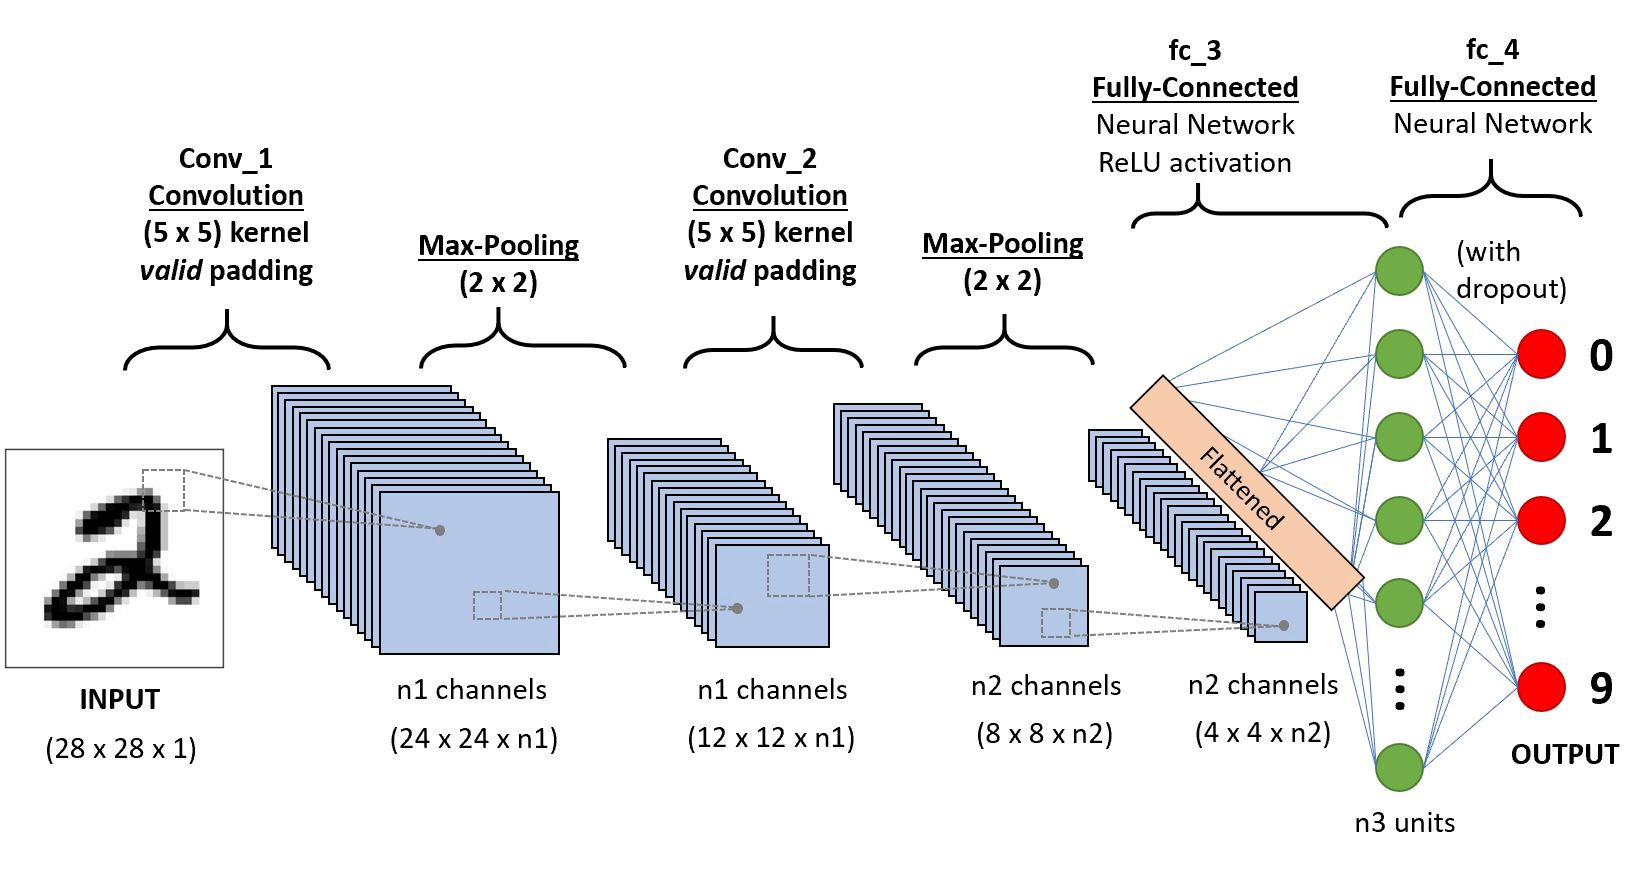
\includegraphics[width=0.7\linewidth]{images/cnn.jpeg}
    %\vspace{1em}
    \caption{Przykładowe architektura sieci splotowej.}
    \label{fig:cnn}
    \source{\url{https://datasciencepr.com/convolutional-neural-network/}}
\end{figure}

Pojedynczy neuron (jednostka obliczeniowa) w sieciach splotowych definiuje się za pomocą:

\begin{itemize}
    \item szerokości,
    \item wysokości,
    \item głębokości (liczba filtrów),
    \item stride (krok przesunięcia filtru) \cite{Forczmanski2020}.
\end{itemize}

\subsection{Podstawowe różnice między sygnałem mowy a sygnałem muzycznym w dziedzinie częstotliwości}
% Tomasz Mąka. Sygnały akustyczne.

Odpowiedź na to pytanie nie była jawnie przedstawiona na wykładach. Jest to raczej wytłumaczone w oparciu o samodzielnie znalezioną wiedzę.
\question

Warto zauważyć, że jest wielka różnorodność jeżeli chodzi o muzykę i mowę. Nie jest proste stworzyć algorytm, który z dobrą skutecznością rozróżniałby te oba sygnały w całych ich dziedzinach. Branie pod uwagę średniej cechy z dziedziny częstotliwości nie jest użyteczne, ponieważ różne przypadki, czy klasy dźwięków mogą znacząco różnić się od wzorca (np. głos Darth'a Vadera)~\cite{hilmar2021speech}.

Jednym ze sposobów rozróżnienia tych klas jest spojrzenie na energię w paśmie poniżej 80Hz. Dla większości sygnałów mowy energia w tym paśmie będzie praktycznie zerowa. W przypadku muzyki z niskimi częstotliwościami (bass, bębny) ten zakres częstotliwości będzie się znacząco różnił~\cite{hilmar2021speech}.

Czyli podsumowując muzyka najczęściej wypełnia całe widmo. Sygnał mowy charakteryzuje się częstotliwościami od 85 Hz do 3kHz.

Jeżeli chodzi o sygnał mowy w dziedzinie częstotliwości to możemy wyznaczać cechy w postaci formantów czy częstotliwości fundamentalnej.

\subsection{Metody próbkowania sieci złożonych}
% Jarosław Jankowski. Sieci złożone.

To jest dziwne, bo to pytanie z przedmiotu \emph{Duże zbiory danych}, które były przedmiotem wspólnym.

Próbkowanie i agregacja dają możliwość rozwiązaniem problemu bardzo dużych zbiorów grafowych. Przykładowo chcąc analizować sieć połączeń na Facebooku, reprezentowaną przez ponad 1 miliard węzłów, potrzebowalibyśmy 1TB pamięci aby zapisać same relacje w postaci grafu, bez atrybutów, etykiet i treści~\cite{Jankowski2020_probkowanie}. 

W próbkowaniu sieci informacja o węzłach jest pozyskiwana dopiero po pobraniu danej próbki, \textbf{struktura całej sieci nie jest znana}. Wymagana jest strategia eksploracji sieci i stopniowego powiększania próbki. Celem próbkowania jest stopniowa identyfikacja małego zbioru przedstawicieli węzłów i powiązań ze struktury sieciowej, przy posiadanej niewielkiej wiedzy o całej sieci. W skrócie jest to uogólnienie sieci, stworzenie modelu sieci, która zachowuje \textbf{niektóre właściwości} sieci pierwotnej~\cite{Jankowski2020_probkowanie}. 

Przy agregacji cała struktura sieci musi być znana apriori. Celem agregacji są miary, które umożliwiają opis własności sieci na poziomie ogólnym~\cite{Jankowski2020_probkowanie}. 

W próbkowaniu sieci homogenicznych (jednorodnych) wyróżniamy dwie główne strategie:

\begin{itemize}
    \item Wybór węzłów lub krawędzi o zadanych właściwościach
    \begin{itemize}
        \item Losowy wybór węzłów
        \item Na podstawie stopnia wierzchołka (prawdopodobieństwo proporcjonalne do stopnia)
        \item Na podstawie miary PageRank
    \end{itemize}
    \item Pobieranie próbek w procesie eksploracji
    \begin{itemize}
        \item Random Walk - rekurencyjnie wybierany losowo tylko jeden z sąsiadów
        \item Snowball sampling - rekurencyjnie włączamy $n$ sąsiadów
        \item Poszukiwanie wzorców
    \end{itemize}
\end{itemize}

W sieciach heterogenicznych (niejednorodnych) możemy skorzystać z \emph{multi-graph sampling}, pobierania próbek z zachowaniem rozkładu typów, próbkowania z zachowaniem relacji~\cite{Jankowski2020_probkowanie}.


\subsection{Elementy składowe procesu klasyfikacji sygnałów akustycznych}
% Tomasz Mąka. Sygnały akustyczne.

Temat ten nie był bezpośrednio podjęty na przedmiocie sygnały akustyczne. Poniższe opracowanie jest zrobione na \textit{chłopski rozum}.
\question

Proces klasyfikacji sygnałów akustycznych składa się z:

\begin{enumerate}
    \item Rejestracji (akwizycji) sygnałów - sygnał jest zapisywany w formie cyfrowej
    \item Wstępne przetwarzanie sygnałów - najczęściej filtrowanie dolnoprzepustowe lub inne procesy mające wyczyścić sygnał (\textit{preprocessing})
    \item Ekstrakcja i selekcja cech - wyznaczamy i wybieramy cechy niezbędne do klasyfikacji. W przypadku podejścia z wykorzystaniem głębokich sieci neuronowych ekstrakcja i selekcja cech wykonywana jest z użyciem takich modeli.
    \item Klasyfikacja - z wykorzystaniem klasyfikatorów, np. liniowych (SVM, LDA), sieci neuronowych (MLP) lub sieci głębokich (jako łącznie z etapem ekstrakcji i selekcji cech)~\cite{jagodzinska2019klasyfikacja}.
\end{enumerate}

\subsection{Model SVM (procedura uczenia, wariant liniowy i nieliniowy, przekształcenia jądrowe).}
% Marcin Korzeń. Uczenie maszynowe 1.

Uczenie liniowego modelu SVM polega na rozwiązaniu \textbf{zadania programowania kwadratowego}:

\begin{equation}
    ||w||^2 \rightarrow \min
\end{equation}

przy liniowych ograniczeniach

\begin{equation}
    d^{(i)}\left(\left\langle w, X^{(i)}\right\rangle+b\right) \geqslant 1, \text { dla } i=1, \ldots, p
\end{equation}

Czyli ma to być znalezienie płaszczyzny z największym marginesem separacji.

W przypadku danych nieseparowalnych liniowo do ograniczeń dodaje się wartość $\varepsilon$. Jest to wariant \emph{soft margin}.

Dla przypadku nieliniowego wykorzystuje się kernel trick, to jest podniesienie wymiarowości danych. Wykorzystanie nieliniowego kernela pozwala stworzyć klasyfikator nieliniowy bez potrzeby przekształcania danych. Algorytm jest formalnie podobny do wariantu liniowego, z wyjątkiem tego, że \textbf{każdy iloczyn skalarny jest zastępowany nieliniową funkcją jądra}. Często wykorzystywanym kernelem jest RBF. 

\subsection{Sieci perceptronowe i metody uczenia perceptronu (warianty algorytmów uczenia, głosowanie, zastosowania)}
% Marcin Korzeń. Uczenie maszynowe 1.

Sieć perceptronowa składa się z pojedynczej warstwy neuronów. Jako funkcja aktywacji wykorzystywana jest bipolarna progowa funkcja aktywacji. Peceptron zbiega w skończonej liczbie iteracji do rozwiązania gdy dane są liniowo separowalne (twierdzenie Novikoffa). Do uczenia perceptronu wykorzystuje się regułę perceptronu \cite{Korzen2020_8}.

 Z matematycznego punktu widzenia wagi perceptronu tworzą wektor normalny, który określa prostą (w przypadku dwóch wejść) lub hiperpłaszczyznę decyzyjną \cite{wiki:Perceptron}.

\begin{figure}[H]
    \centering
    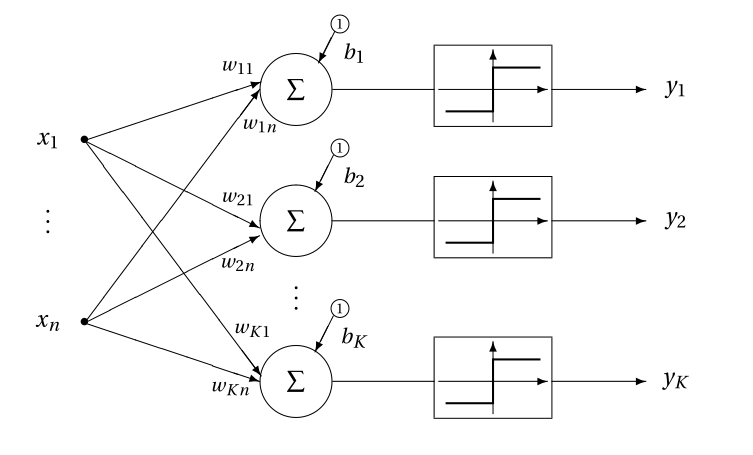
\includegraphics[width=0.5\linewidth]{images/perceptron.png}
    \caption{Wizualizacja perceptronu.}
    \label{fig:apriori}
    \source{Uczenie Maszynowe 1, Wykład VII - Perceptron \cite{Korzen2020_8}}
\end{figure}

Uczenie perceptronu przebiega zgodnie z \textbf{regułą perceptronu}. W skrócie, polega ona na korygowaniu wag w przypadku gdy próbka została źle sklasyfikowana. 

Inne warianty uczenia perceptronu to uczenie perceptronu z $\gamma$-marginesem, voted perceptron czy average perceptron.

Wariant z $\gamma$-marginesem polega na tym, że wagi są korygowane wtedy gdy próbka przekracza obrany margines (nie jak wcześniej czy jest źle klasyfikowana).

\textbf{Perceptron z głosowaniem} polega na tworzeniu wielu perceptronów (zestawów wag). Dla każdego zestawu wag przechowywany jest licznik, który opisuje ile próbek zostało dobrze sklasyfikowanych aż wagi należało poprawić. W procesie predykcji wybieramy głosem większościowym odpowiedzieć klasyfikatora. W \textbf{wersji average perceptron} różnica występuje tylko w odpowiedzi klasyfikatora. Gdzie wybierana jest średnia ze wszystkich klasyfikatorów.
\question

\subsection{Proces tworzenia zbioru uczącego, walidującego i testowego w głębokim uczeniu}
% Paweł Forczmański. Uczenie maszynowe 2.

Przygotowanie zbioru danych jest niezbędne w uczeniu maszynowym. Zbiór danych najczęściej jest podzielony na zbiór uczący, zbiór testowy i zbiór walidujący. 

Zbiór uczący jest wykorzystywany do uczenia modelu. Jest on największy ze wszystkich. Przede wszystkich w głębokim uczeniu wymagane są duże ilości próbek uczących.

Zbiór walidujący wykorzystywany jest do testowania na etapie tworzenia i implementacji modeli. Wykorzystywany jest to oceniania modeli z różnymi hyperparametrami. 

Zbiór testowy powinien zostać użyty tylko raz, na końcu całego procesu implementacji modelu. Wykorzystywany jest do przetestowania skuteczności stworzonego rozwiązania. 

W przypadku braku wystarczającej liczby danych uczących można korzystać z kroswalidacji. Wykorzystuje się ją najczęściej w metodach klasycznych. W głębokim uczeniu metoda kroswalidacji nie jest wykorzystywana ze względu na długie czasy uczenia modeli.

W głębokim uczeniu rozmiar próby uczącej powiększa się za pomocą augmentacji. W przypadku obrazów może to być odbijanie w poziomie, rozjaśnianie, kadrowanie, itd.

\subsection{Sposób działania algorytmów uczących AdaBoost i RealBoost}
% Przemysław Klęsk. Uczenie maszynowe 2.

Algorytmy z rodziny boosting polegają na reważeniu przykładów uczących. Ich zasadniczą cechą jest odporność na przeuczenie.

Klasyfikator boosting składa się z wielu słabych klasyfikatorów. Najczęściej łączy się je z \emph{decision stump} (zdegenerowane drzewo decyzyjne), lub innymi wariantami klasyfikatorów (drzewa decyzyjne, SVM, naiwny Bayes) \cite{Klesk2020}.

Uczenie klasyfikatora składa się z wielu rund. W każdej iteracji uczony jest słaby klasyfikator na danych uczących używając ważonych przykładów. Wagi przykładów aktualizuje się tak, że najważniejsze stają się próbki źle sklasyfikowane \cite{Klesk2020}.

W pojedynczej rundzie wybór słabego klasyfikatora odbywa się teoretycznie według dowolnie obranego kryterium błędu. Najczęściej rozważa się minimalizację błędu klasyfikacji lub minimalizację kryterium wykładniczego \cite{Klesk2020}.

Wystarczy że słabe klasyfikatory będą dawać odpowiedzi różne od 0.5. Gdy dokładność klasyfikatora jest mniejsza niż 0.5 to odpowiedź klasyfikatora jest negowana.

Rozwinięciem AdaBoost jest RealBoost. Słabe klasyfikatory są rzeczywistoliczbowe a nie binarne jak w Adaboost. Odpowiedź słabego klasyfikatora jest zwykle ustalana jako przybliżenie połowy przekształcenia logit. Rezygnuje się ze współczynników ważących słabe klasyfikatory. Mechanizm ważenia klasyfikatorów jest wpleciony w same odpowiedzi rzeczywistoleiczbowe \cite{Klesk2020}.
\question


\subsection{Omówienie na przykładzie algorytmu Apriori odkrywania asocjacji w zbiorach danych}
% Joanna Kołodziejczyk. Eksploracja danych.

Algorytm Apriori opiera się na własności, że wszystkie podzbiory częstego zbioru przedmiotów również muszą być częste. Przykładowo, w transakcjach często występuje reguła: bułka, ser żółty, pomidor $\rightarrow$ szynka, to wszystkie elementy tej reguły też często występują w zbiorze transakcji \cite{Kolodziejczyk2020}.

Algorytm Apriori jest przeznaczony do znajdowania wzorców w dużych zbiorach danych. Jeśli jakiś wzór występuje często, to jest on uważany za ,,interesujący'' \cite{Kolodziejczyk2020}.

Algorytm składa się z dwóch etapów: znajdowania częstych wzorców z wykorzystaniem progu minimalnego wsparcia, oraz znajdowaniem odpowiednich reguł z progiem minimalnego zaufania. Generowanie kandydatów do wzorców można przeprowadzić metodą brute-force, albo metodami $F_{k-1} \times F_1$, lub $F_{k-1} \times F_{k-1}$. Metoda brute-force nie sprawdzi się w bardzo dużych zbiorach danych.

\begin{figure}[H]
    \centering
    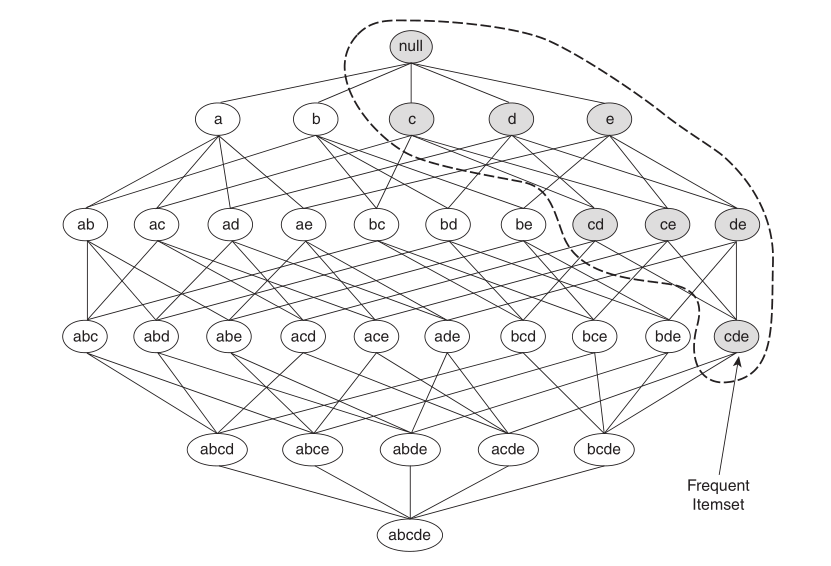
\includegraphics[width=0.5\linewidth]{images/apriori.png}
    \caption{Przedstawienie reguły Apriori. Jeżeli zbiór $\{c, d, e\}$ jest częsty, to wszystkie podzbiory też są częste.}
    \label{fig:apriori}
    \source{\url{https://www-users.cs.umn.edu/~kumar001/dmbook/ch5_association_analysis.pdf}}
\end{figure}


Na początku tworzymy zbiór potencjalnych wzorców jednoelementowych z danym progiem wsparcia. Wyszukiwanie przeprowadzamy iteracyjnie zwiększając wielkości zbiorów. 

Mając wygenerowane potencjalne wzorce z pierwszego kroku należy wygenerować reguły z zaufaniem większym niż ustalony minimalny próg wsparcia. Wygenerowane reguły należy posortować malejąco na podstawie metryki \emph{lift}.

\subsection{Przykład sieci bayesowskiej (przekonań): struktura sieci, właściwości i jej interpretacja oraz uczenie}
% Joanna Kołodziejczyk. Eksploracja danych.

Sieć Bayesowska (sieć przekonań) jest probabilistycznym modelem grafowym, który reprezentuje zbiór zmiennych i ich zależności warunkowych za pomocą acyklicznego grafu. Sieci Bayesowskie są dobre do przewidywania zdarzeń zależnych (obliczania \emph{likelihood} \cite{wiki:Likelihood_function}) na podstawie zdarzenia zaobserwowanego 
\cite{wiki:Bayesian_network}. Przykładowo mamy sieć przedstawioną na rysunku \ref{fig:bayesian}. Na podstawie różnych przesłanek Holmes ma zdecydować czy wracać do domu z powodu włamania. Są to: alarm, telefon od Watsona, trzęsienie ziemi i informacja w wiadomościach o trzęsieniu.


\begin{figure}[H]
    \centering
    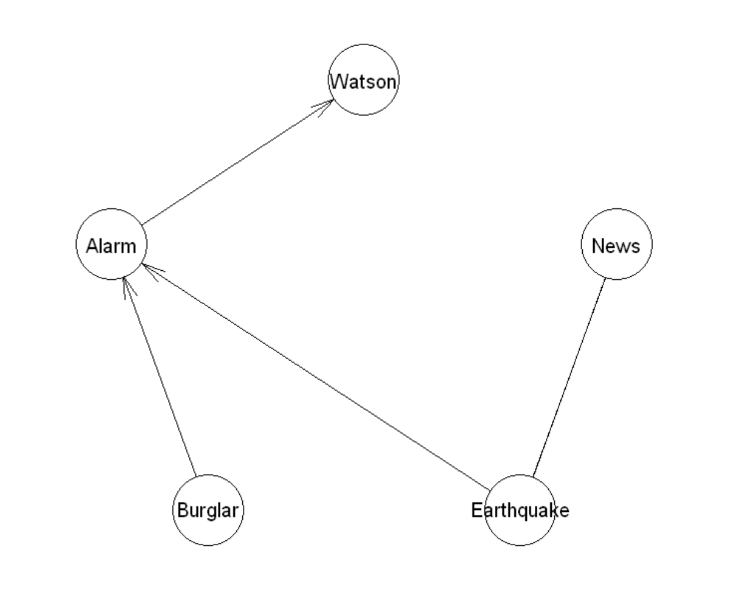
\includegraphics[width=0.5\linewidth]{images/bayesian.png}
    \caption{Przykład sieci Bayesowskiej}
    \label{fig:bayesian}
    \source{Opracowanie własne}
\end{figure}


Na laboratorium wykorzystywaliśmy bibliotekę \emph{bnlearn}\footnote{\url{https://www.bnlearn.com/documentation/man/bn.fit.html}} do tworzenia sieci i ich uczenia. Aby nauczyć sieć wprowadzaliśmy prawdopodobieństwa warunkowe zdarzeń.
\question

\subsection{Deskryptory cech niskopoziomowych - wybrane algorytmy w odniesieniu do wykorzystywanych cech}
% Dariusz Frejlichowski. Ekstrakcja cech.

Deskryptory cech odnoszą się do zagadnienia ekstrakcji cech. Deskryptor opisuje daną cechę za pomocą wartości numerycznych. Poniżej opisano tylko deskryptory odnoszące się do obrazów. Oprócz tego istnieją inne deskryptory, np. w rozpoznawaniu dźwięku częstotliwość fundamentalna, formanty, itd.

\textbf{Atrybuty niższego poziomu abstrakcji} - metadane typu sygnałowego, są wartościowane przez komputer (np. kolor dominujący, histogram krawędzi, aktywność ruchu w obrazie, czy linia melodyczna utworu muzycznego) \cite{Frejlichowski2020}.

Standard MPEG-7 opisuje między innymi deskryptory wizualne. Deskryptory wizualne MPEG-7 opisują na \textbf{niewielu} bitach obrazy, sekwencje obrazów, obszary w obrazie itd. 

Deskryptor powinien być:

\begin{itemize}
    \item efektywny i ekspresyjny (porównywalny z widzeniem u ludzi),
    \item zwarty (w aspekcie pamięci),
    \item o małej złożoności ekstrakcji i zapytań \cite{Frejlichowski2020}.
\end{itemize}

Wyróżniamy następujący podział deskryptorów:

\begin{itemize}
    \item \textbf{Koloru} - Scalable Color, Color Structure, Dominant Color, histogramy,
    \item \textbf{Kształtu} - sygnatura, UNL, UNL-F, mUNL,
    \item \textbf{Odcieni szarości} - Polar-Fourier Greyscale Descriptor, Rzutowanie wartości,
    \item \textbf{Ruchu},
    \item \textbf{Tekstury}.
\end{itemize}

\subsubsection{Deskryptory kształtu}

Główne problemy z deskryptorami kształtu to:

\begin{itemize}
    \item obrót, skalowanie, przesunięcie (przekształcenia afiniczne)
    \item szum,
    \item nieciągłości,
    \item okluzja.
\end{itemize}

Czyli najlepszy deskryptor jest inwariantny względem obrotu, skalowania, przesunięcia oraz jest niewrażliwy na szum i okluzję.

Proste deskryptory kształtu to m.in. pole powierzchni, długość obwodu, kołowość, zwartość, mimośród, powłoka wypukła, object aspect ratio, itd. \cite{Frejlichowski2020_2}

Przykładowym deskryptorem jest UNL-F. Zapewnia on dobrą odporność na szum, przekształcenia afiniczne (transformata Fouriera daje odporność na obrót). Jedyną wadą jest brak odporności na okluzję. W pewnym stopniu rozwiązuje to mUNL, który zmienia podejście do wyznaczania centroidu  \cite{Frejlichowski2020_2}.

W skrócie UNL-F składa się on z następujących kroków:

\begin{enumerate}
    \item Binaryzacja obiektu
    \item Wyznaczenie centroidu
    \item Przekształcenie do współrzędnych polarnych
    \item Wycinek widma po transformacie 2D Fouriera -- tego kroku nie ma w zwykłej metodzie UNL
\end{enumerate}

\begin{figure}[H]
    \centering
    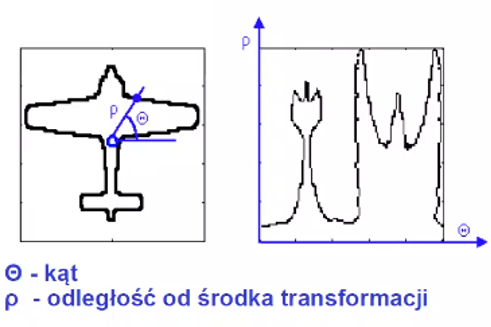
\includegraphics[width=0.5\linewidth]{images/unl.png}
    \caption{Działanie deskryptora UNL}
    \label{fig:unl}
    \source{Wykład 2 - D. Frejlichowski \cite{Frejlichowski2020_2}}
\end{figure}

\subsubsection{Deskryptory koloru}

Przykładowe deskryptory koloru ze standardu MPEG-7 to:

\begin{itemize}
    \item Deskryptor koloru dominującego
    \item Skalowalny deskryptor koloru
    \item Deskryptor GOF i GOP
    \item Deskryptor struktury koloru
    \item Deskryptor widoku koloru (layout)
    \item Temperatura barwowa \cite{Frejlichowski2020_6}
\end{itemize}

Inne deskryptory koloru to:

\begin{itemize}
\item histogram RGB lub HSV - może dawać takie same wyniki dla różnych obrazów
\item IBOX8
\item DHV
\item RGBBOX8
\item RGBI \cite{Frejlichowski2020_6}
\end{itemize}

Przykładowo, deskryptor koloru dominującego polega na wyznaczenie $n$ kolorów dominujących dla obrazu za pomocą algorytmu $k$-means i obliczenie ich udziałów \cite{Frejlichowski2020_6}.

Skalowalny deskryptor koloru bazuje na przestrzeni barw HSV i transformacji Haara zastosowanej na wartościach histogramu koloru \cite{Frejlichowski2020_6}.

Deskryptor rozkładu koloru (Color Layout Descriptor) uchwyca rozkład przestrzenny kolorów w bazie. Polega na transformacji DCT dla poszczególnych składowych w przestrzeni YcbCr~\cite{Frejlichowski2020_6}.

\subsubsection{Deskryptory odcieni szarości}

W pewnym sensie deskryptory odcieni szarości łączą w sobie deskryptory kolorów i kształtu. Przykładowym deskryptorem jest Polar-Fourier Grayscale Descriptor.

Polega on na wstępnym preprocessingu (filtry), wyznaczeniu centroidu obrazu w skali szarości, transformacji obrazu do współrzędnych biegunowych i wycięciu fragmentu widma po transformacie 2D Fouriera \cite{frejlichowski2015application}.

Alternatywny deskryptor polegał na przekształceniu biegunowym i rzutowaniu wartości. Rzutowanie to suma po kolumnach i suma po wierszach. Taki deskryptor daje na wyjściu dwa wektory. Dawał gorsze wyniki niż PFGD \cite{Frejlichowski2020_5}.


\subsection{Główne miary centralności w sieciach złożonych}
% Jarosław Jankowski. Sieci złożone.

Sieci złożone to nic innego jak rozbudowane grafy służące np. do modelowania społeczności, węzłów komunikacyjnych, infrastruktury itd. Mogą występować grafy skierowane lub nieskierowane.

\textbf{Miary centralności} wyznaczają najważniejsze węzły w grafie ze względu na różne własności~\cite{Jankowski2020}. Wyróżniamy następujące miary:

\begin{itemize}
    \item Degree - stopień wierzchołka
    \item Betweenness - ile razy węzeł stanowi pomost jako element najkrótszej ścieżki pomiędzy innymi węzłami sieci
    \item Closeness - średnia długość najkrótszej ścieżki między węzłem, a wszystkimi innymi węzłami. Bardziej centralne węzły mają bliżej do wszystkich innych węzłów w sieci.
    \item PageRank - zliczanie liczby i jakości linków do węzłów aby określić ważność węzła. Podstawowym założeniem jest to, że ważne węzły otrzymują więcej połączeń z innych ważnych węzłów.
    \item Eigenvector
\end{itemize}

\subsection{Pakiety języka Python wykorzystywane w analizie danych}
% Marcin Pluciński. Języki analizy danych.

Najpopularniejsze pakiety Pythona wykorzystywane w analizie danych to:

\begin{itemize}
    \item \textbf{numpy} - wielowymiarowe macierze i operacje na tych strukturach
    \item \textbf{scipy} - optymizacja, algebra liniowa, interpolacja, FFT, przetwarzanie sygnałów itd.
    \item \textbf{pandas} - przetwarzanie danych i analiza. Struktury danych do manipulowania tabelami i szeregami czasowymi.
    \item \textbf{matplotlib} - biblioteka do wizualizacji
    \item \textbf{geopandas} - odpowiednik pandas (rozszerzenie) do danych przestrzennych
    \item \textbf{sklearn} (scikit learn) - implementacje modeli uczenia maszynowego
\end{itemize}

\subsection{Techniki regularyzacji modeli klasyfikacyjnych i regresyjnych (regularyzacja L1, L2, elastic net; problemy optymalizacyjne; zastosowania)}
% Marcin Korzeń. Uczenie maszynowe 1.

Ogólne podejście do problemu uczenia można zdefiniować następująco:

\begin{equation}
    Q(\theta \mid \mathscr{D})=L(\theta \mid \mathscr{D})+\gamma R(\theta)
\end{equation}

gdzie:

\begin{description}
\item[L(\theta \mid \mathscr{D})] to funkcja straty, błędu, dopasowanie modelu do danych,
\item[R(\theta)] to kara za złożoność modelu,
\item[\gamma] ustala kompromis pomiędzy dopasowaniem, a złożonością.
\end{description}

Regularyzacja to modyfikacja modelu, np. przez dodanie kary za złożoność, która ma na celu zmniejszenie błędu testowego zapobiegając zjawisku przeuczenia \cite{wiki:Regularization}.

Regularyzacja jest konieczna gdy:

\begin{itemize}
    \item mamy pewną wiedzę na temat możliwych rozwiązań,
    \item niejednoznaczność rozwiązania,
    \item numeryczna niestabilność algorytmów \cite{Korzen2020_12}.
\end{itemize}
\question

\textbf{Regularyzacja typu $L^1$ (lasso)} w modelach klasyfikacyjnych i regresyjnych stosujemy aby poprawić własności numeryczne algorytmów oraz gdy zależy nam na selekcji zmiennych w trakcie uczenia. Modele z taką regularyzacją są rzadkie, to znaczy, współczynniki przy wielu atrybutach są zerowe. Jest to zjawisko dobre w przypadku, gdy chcemy dokonać selekcji zmiennych -- mało jest atrybutów istotnych i dużo szumu.

\textbf{Regularyzacja typu $L^2$ (ridge)} w modelach klasyfikacyjnych i regresyjnych również stosujemy aby poprawić własności numeryczne algorytmów oraz w przypadkach, gdy dane zawierają wiele zmiennych skorelowanych.

Model ElasticNet łączy regularyzację $L^1$ oraz regularyzację $L^2$ \cite{wiki:Elastic_net_regularization}. 

Nie wiem jakie są problemy optymalizacyjne tych technik regularyzacji.
\question

Podsumowując:

\begin{itemize}
    \item składnik straty $L(\theta \mid \mathscr{D})$ jest mniej istotny,
    \item składnik związany z regularyzacją $R(\theta)$ prowadzi do różnych jakościowo modeli,
    \item $L^1$ jest dobry, gdy mało jest atrybutów istotnych i dużo szumu (bardzo dobry mechanizm selekcji), oraz gdy jest mało danych,
    \item $L^2$ jest dobry, gdy dużo jest atrybutów istotnych i dużo korelacji \cite{Korzen2020_12}.
\end{itemize}

\printbibliography[heading=bibintoc]

% \appendix

% \section{Przykłady do kopiowania}

% \begin{table}[H]
% \caption{Czas trwania jednej epoki dla rozmiaru obrazu}
% \vspace{1em}
% \centering
% \begin{tabular}{@{}lr@{}}
% \toprule
% Rozmiar          & Czas {[}s{]} \\ \midrule
% $32 \times 32$   & 0.1288       \\
% $64 \times 64$   & 0.2000       \\
% $128 \times 128$ & 1.046        \\ \bottomrule
% \end{tabular}
% \end{table}

% \code{Przykład kodu}
% {Opracowanie własne}{\label{kod:przyklad}}
% \begin{lstlisting}[language=Python]
% discriminator = make_discriminator_model()
% generator = make_generator_model()
% \end{lstlisting}

% \begin{figure}[H]
%     \centering
%     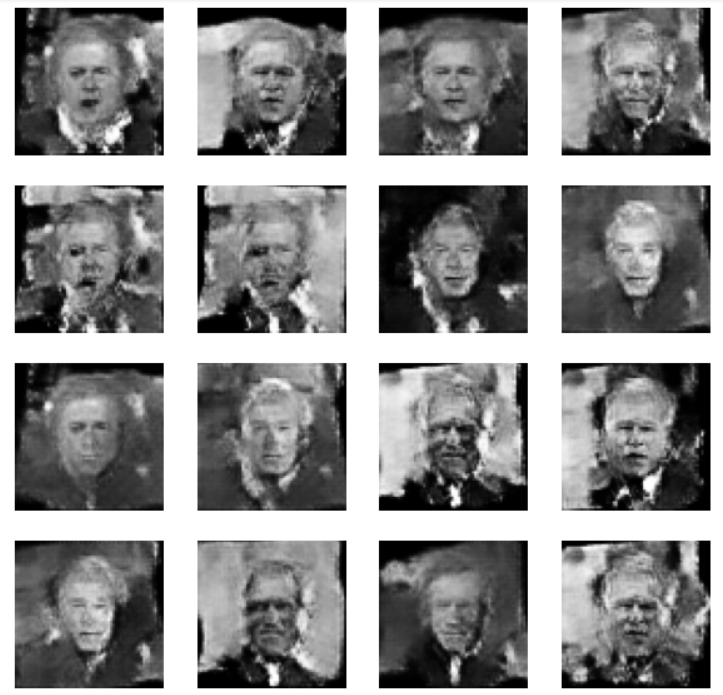
\includegraphics[width=0.7\linewidth]{images/sample.png}
%     %\vspace{1em}
%     \caption{Przykładowy obrazek}
%     \label{fig:pdgd}
%     \source{Opracowanie własne}
% \end{figure}


\end{document}
